% Created 2019-12-23 Mon 23:19
% Intended LaTeX compiler: pdflatex
\documentclass{article}
\usepackage[utf8]{inputenc}
\usepackage[T1]{fontenc}
\usepackage{graphicx}
\usepackage{grffile}
\usepackage{longtable}
\usepackage{wrapfig}
\usepackage{rotating}
\usepackage[normalem]{ulem}
\usepackage{amsmath}
\usepackage{textcomp}
\usepackage{amssymb}
\usepackage{capt-of}
\usepackage{hyperref}
\usepackage[cachedir=/tmp/minted]{minted}
\usepackage[round]{natbib}
\bibliographystyle{abbrvnat}
\newcommand{\dbatversion}{0.9.1.2}
\newcommand{\dbatdate}{Dec 09, 2019}
\setcounter{secnumdepth}{4}
\usepackage{authblk}
\author[1]{Niclas Börlin}
\author[2]{Pierre Grussenmeyer}
\affil[1]{Department of Computing Science, Ume{\aa} University, Sweden, \texttt{niclas.borlin@cs.umu.se}}
\affil[2]{ICube Laboratory UMR 7357, Photogrammetry and Geomatics Group, INSA Strasbourg, France, \texttt{pierre.grussenmeyer@insa-strasbourg.fr}}
\newcommand{\contributions}{%
With contributions from:%
\begin{itemize}
\item Arnaud Durand, ICube-SERTIT, University of Strasbourg, France.
\item Jan Hieronymus, TU Berlin, Germany.
\item Jean-Fran{\c{c}}ois Hullo, EDF, France.
\item Fabio Menna, Fondazione Bruno Kessler, Trento, Italy.
\item Arnadi Murtiyoso, ICube, INSA Strasbourg, France.
\item Kostas Naskou, University of Nottingham, UK.
\item Erica Nocerino, Fondazione Bruno Kessler, Trento, Italy.
\item Deni Suwardhi, Bandung Institute of Technology, Indonesia.
\end{itemize}
}

\newmintinline{xml}{}

\date{\dbatdate}
\title{DBAT --- The Damped Bundle Adjustment Toolbox for Matlab\\\medskip
\large v\dbatversion}
\hypersetup{
 pdfauthor={},
 pdftitle={DBAT --- The Damped Bundle Adjustment Toolbox for Matlab},
 pdfkeywords={},
 pdfsubject={},
 pdfcreator={Emacs 25.2.2 (Org mode 9.2.6)}, 
 pdflang={English}}
\begin{document}

\maketitle
\setcounter{tocdepth}{4}
\contributions \newpage \tableofcontents \clearpage
\section{Introduction}
\label{sec:org59d8c85}
\subsection{Purpose}
\label{sec:org0e78491}
The purpose of the Damped Bundle Adjustment toolbox is to be a
high-level toolbox for photogrammetry in general and bundle adjustment
in particular. It is the hope of the authors that the high-level
nature of the code will inspire algorithm development. The code is
written in Matlab and is verified to work with Matlab version 9.5
(release R2018b). The intention is that at least the computation
routines will be Octave-compatible. This has however not been tested
yet.

\subsection{Contents}
\label{sec:org3f0db5c}
\subsubsection{XML scripts}
\label{sec:orgaf776c2}

As of DBAT version 0.9, DBAT can be used via an XML interface or a
direct Matlab interface. The XML interface allows usage without much
Matlab knowledge, see Section~\ref{sec:xml} and
\citet{Borlin2019:Implementing}.

\subsubsection{Matlab code}
\label{sec:org5de1726}
The toolbox currently includes routines for (Matlab function names in
parentheses):
\begin{itemize}
\item File handling:
\begin{itemize}
\item Reading PhotoModeler-style text export files (\texttt{loadpm}), and 2D/3D
point table exports files (\texttt{loadpm2dtbl} and \texttt{loadpm3dtbl},
respectively).
\item Reading PhotoScan native (.psz) files (\texttt{loadpsz}).
\item Writing PhotoModeler-style text result files
(\texttt{bundle\_result\_file}).
\end{itemize}
\item Post-processing:
\begin{itemize}
\item Post-processing of PhotoScan projects (\texttt{ps\_postproc}). Includes
object point filtering on low ray count and low intersection
angles. For self-calibration post-processing, see the help text
for \texttt{ps\_postproc}.
\item As of version 0.7.0.0, DBAT supports both lens distortion models
used by Photomodeler and Photoscan.
\end{itemize}
\item Photogrammetric calculations, including:
\begin{itemize}
\item Spatial resection (\texttt{resect}).
\item Forward intersection (\texttt{forwintersect}).
\item Absolute orientation (\texttt{rigidbody}).
\item Relative orientation based on the Nistér 5-point algorithm
\citep{Stewenius2006:Recent} will be added in the future.
\end{itemize}
\item Bundle adjustment proper (\texttt{bundle}):
\begin{itemize}
\item With or without self-calibration.
\item Works with fixed or weighted prior observations, e.g., control
points.
\item Works with prior observations of camera positions.
\item Supports check points.
\item What parameters that should be estimated are selectable at the
parameter level, e.g. down to the coordinate level for 3D points.
\item Estimated parameters can be block-invariant (the same for a whole
block), image-variant (individual for each image), or anything
inbetween. Parameter sets may be split-variant, e.g., with some IO
parameters block-invariant and some IO parameters image-variant
\citep{Borlin2019:Flexible}.
\item \sloppy Uses either Classical Gauss-Markov, Gauss-Newton-Armijo,
Levenberg-Marquardt, or Levenberg-Marquardt-Powell damping schemes
\citep{Borlin2013:Bundle,Borlin2014:Camera,Borlin2016:External}.
\item Posterior covariance calculations (\texttt{bundle\_cov}) from the bundle
result, including correlations and significance levels, point and
image quality statistics.
\end{itemize}
\item Analysis of camera networks, including:
\begin{itemize}
\item Detection of structural rank deficiency (Matlab's \texttt{dmperm},
\texttt{sprank}). Useful as a sanity check on input data. Structural rank
deficiency is typically caused by trying to estimate a parameter
with too few direct observations.
\item Null-space analysis if the normal matrix is singular using
\texttt{spnrank} \citep{Foster2009:Calculating}. This might, e.g., be
caused by insufficient datum specification.
\end{itemize}
\sloppy The result of the analysis, including suggestions for what
parameters may be impossible to estimate are written to the report
file by \texttt{bundle\_result\_file}.
\item Various plotting functions, including:
\begin{itemize}
\item Plot image covered by measurements (\texttt{plotcoverage}).
\item Plot camera network (\texttt{plotnetwork}), either static (as-loaded) or
as an illustration of the bundle iterations.
\item Plot .psz project (\texttt{loadplotpsz}).
\item Plot of the iteration trace of parameters estimated by bundle
(\texttt{plotparams}).
\item Plots of quality statistics from the bundle result
(\texttt{plotimagestats, plotopstats}).
\end{itemize}
\item Demo functions using the above functions. The demo functions are
detailed in Section~\ref{sec:demos}. The available demos are listed
by executing the command \texttt{help dbatdemos}. This manual does not
contain detailed information about how to use each function. More
information may be found by typing \texttt{help <function name>} at the
Matlab prompt, studying the source code of the demo functions, and
reading the source code of each file directly.
\item XML scripts that allow a user to tailor the computation without
writing any Matlab code (\texttt{rundbatscript}), see
Section~\ref{sec:xml} and \citet{Borlin2019:Implementing}.
\end{itemize}

\subsubsection{Data}
\label{sec:org89bc19c}
The toolbox contains several datasets, including datasets for the
\citet{Borlin2016:External,Murtiyoso2017:Reprocessing} papers.

\begin{itemize}
\item PhotoModeler export files or PhotoScan projects.
\item Images. To reduce the size of the distribution package, only low
resolution images are included in the package \footnote{No images are included in the StPierre data set.}. The
corresponding high resolution images can be downloaded from
\url{http://people.cs.umu.se/niclas/dbat_images}. Further instructions
are found in \texttt{README.txt} files in the respective image directories.
\end{itemize}

The simplest way to access the data sets is through the XML scripts,
described in Section~\ref{sec:xml}, or through the demos, described in
Section~\ref{sec:demos}.

\subsection{Legal}
\label{sec:orgd051164}

The licence detail are described in the \texttt{LICENSE.txt} file included in
the distribution and in Appendix~\ref{sec:license}. In summary:

\begin{itemize}
\item You use the code at your own risk.
\item You may use the code for any purpose, including commercial, as
long as you give due credit. Specifically, if you use the code, or
derivatives thereof, for scientific publications, you should refer
to on or more of the papers
\citet{Borlin2013:Bundle,Borlin2013:Experiments,Borlin2014:Camera,Borlin2016:External,Borlin2018:Modular,Borlin2019:Implementing,Borlin2019:Flexible}
that the code is based on.
\item You may modify and redistribute the code as long as the
licensing details are also redistributed.
\end{itemize}

\newpage
\section[Installation]{Installation (from the file INSTALL.txt)}
\label{sec:install}
\begin{minted}[autogobble,fontsize=\tiny,frame=single,fontsize=\small,frame=none]{text}
# == INSTALLATION ==
#
# You can either install DBAT by downloading the source code or (if
# you use a git client) by cloning the repository.
#
# === Download ===
#
# 1) Download the package file dbat-master.zip (from the main page) or
#    dbat-x.y.z.w.zip/dbat-x.y.z.w.tar.gz (from the releases page) of
#    https://github.com/niclasborlin/dbat/
#
# 2) Unpack the file into a directory, e.g., c:\dbat or ~/dbat.
#
# === Clone ===
#
# At the unix/windows command line, write:
#
#   git clone https://github.com/niclasborlin/dbat.git
#
# to clone the repository into the directory 'dbat'. Use
#
#   git clone https://github.com/niclasborlin/dbat.git <dir-name>
#
# to clone the repository to another directory.
#
# If you use a graphical git client, e.g., tortoisegit
# (https://tortoisegit.org), select Git Clone... and enter
# https://github.com/niclasborlin/dbat.git or
# git@github.com:niclasborlin/dbat.git as the URL.
#
#
# ==== Download high-resolution images ====
#
# To reduce the size of the repository and hence download times, only
# low-resolution images are included in the repository. High-resolution 
# images can be downloaded from http://people.cs.umu.se/niclas/dbat_images/.
# For further details, consult the README.txt files in the respective
# image directories.
#
#
# == TESTING THE INSTALLATION ==
#
# 1) Start Matlab. Inside Matlab, do the following initialization:
# 1.1) cd c:\dbat % (change to where you unpacked the files)
# 1.2) dbatSetup  % will set the necessary paths, etc.
#
# 2) To test the demos, do 'help dbatdemos' or consult the manual.
#
#
# == UPDATING THE INSTALLATION==
#
# === Git ===
#
# If you cloned the archive, updating to the latest release is a
# simple as (replace ~/dbat and c:\dbat with where you cloned the
# repository):
#
#   cd ~/dbat
#   git pull
#
# at the command line. In TortoiseGit, right-click on the folder
# c:\dbat, select Git Sync... followed by Pull.
#
# === Download ===
#
# If you downloaded the code, repeat the download process under
# INSTALLATION. Most of the time it should be ok to unzip the new
# version on top of the old. However, we suggest you unzip the new
# version into a new directory, e.g., dbat-x-y-z-w, where x-y-z-w is
# the version number.
#
#
\end{minted}

\newpage
\section[Change log]{Change log (from the file ChangeLog.txt)}
\label{sec:changeLog}
\begin{minted}[autogobble,fontsize=\tiny,frame=single,fontsize=\small,frame=none]{text}
Summary changelog file for release.

Release 0.9.1.2, Dec 09, 2019.
- Hide internal sign flip for some camera parameters.
- Add change log to the manual.

Release 0.9.1.1, Dec 07, 2019.
- Updated manual to include DBAT XML scripts.
- Added UUID tags.

Release 0.9.1.0, Dec 02, 2019.
- First public support for DBAT XML scripts.
- Reorganization of data files.

Release 0.9.0.1, Nov 22, 2019.
- Internal release with full operations and plotting support and file output
  except IO.

Release 0.9.0.0, Nov 16, 2019.
- Internal release with nominal support for DBAT XML scripts.
- Scripting support for input (full), operations (most), output (minor).

Release 0.8.5.1, Jan 13, 2019.
- Fix to avoid some lengthy pre-bundle computations unless they are needed.

Release 0.8.5.0, Jan 03, 2019.
- Major restructuring of the main data structure.
- Added support for prior observations of camera positions.
- Added high-level functions to refer to camera parameters by name
  rather than by row number.
- Added high-level functions to set up EO/OP parameters for the bundle.
- Added more information about computer system to report file.
- Added information about control files to report file.
- Cleaned up naming scheme of camera parameters.
- Various bugfixed, including handling of overlapping normal and
  smartpoint ids in PM export file.

Release 0.8.0.0, Oct 26, 2018.
- Parameter handling in bundle rewritten to allow parameters to be
  estimated to be block-invariant (common to all images),
  image-variant (unique for each image), and anything inbetween.
  Furthermore, parameter sets can be split-variant, e.g., some IO
  parameters can be block-invariant and some can be image-variant.
- Added cumulative significance computation for lens K and P
  parameters to the result file.
- Added parameter and observation count and total redundancy to the
  result file.

Release 0.7.6.1, Oct 25, 2018.
- Bugfix to v0.7.6.0 to fix that the format change was introduced with
  Photoscan v1.4.1 and not with v1.4.0.

Release 0.7.6.0, Oct 17, 2018.
- Added support for Photoscan file format v1.4.0 (Photoscan program v1.4.x).

Release 0.7.5.0, May 30, 2018.
- Restructured Jacobian computations for Riva 2018 conference paper.
- Added support for affine parameters (aspect and skew) (lens distortion
  models 3-5).
- Bugfixes to generate report file also when bundle fails.
- Added absolute termination criteria - useful when testing on
  synthetic data without errors.
- Added sanity check of input problem based on structural rank
  (Dulmage-Mendelsohn permutations) to detect if any parameter is
  impossible to estimate due to too few observations.
- Added null-space analysis if normal matrix is singular to suggest
  what parameters are linearly dependent. Uses spnrank function by
  Leslie Foster, Math Dept., San Jose State University.
- Added example demos with missing observations or no datum.
- Updated manual with descriptions of the error detection demos.

Release 0.7.0.4, Dec 28, 2017.
- Bugfixes and updated instructions.
- Removed unintended reliance on the Statistical Toolbox (nanmean function).
- Improved error messages and testing of loading problems for
  Photomodeler export files reported by some users.
- Added a loadpm bugfix that showed up in early (pre-R2015b) Matlab
  versions only. Bugfix provided by Fabio Menna.
- Updated INSTALL.txt with instructions for git cloning and DBAT updates.
- Added file BUGREPORTS with instructions how to submit a bug report
  and/or feature request.

Release 0.7.0.3, Dec 27, 2017.
- Internal release for testing only.

Release 0.7.0.2, Dec 27, 2017.
- Bugfixes, including removing spurious incorrect warning for
  non-local coordinate system in .psz file.

Release 0.7.0.1, Nov 29, 2017.
- Various bugfixes.
- Now ignores disabled and unoriented cameras in .psz project files.
- Added warning for non-local coordinate system in .psz file.

Release 0.7.0.0, Nov 24, 2017.
- Public release of version with StPierre test data and support for
  Forward Brown (Computer Vision/Photoscan) lens distortion model.

Release 0.6.5.5, Oct 16, 2017.
- Bugfixes.
- Added computation and printout of rigid-body transformation for
  ctrl/check pts to detect mismatches between ctrl pt file and projects.
- Added cleaned (no image info) StPierre .psz file.
- Added ray count printout for ctrl/check pts in result file.
- Fixed scaling of PS lens distortion coordinates.

Release 0.6.5.0, Oct 12, 2017.
- Added automatic support for check points. Ctrl pts found in the
  control point file but not used as ctrl pts in the PM/PS project are
  used as check points.
- Added printout of prior and posterior ctrl pts estimates.

Release 0.6.4.3, Oct 11, 2017.
- Added loading of external ctrl pts for the StPierre data set.

Release 0.6.4.2, Oct 6, 2017.
- General performance increase, especially with self-calibration.

Release 0.6.4.1, Oct 5, 2017.
- Performance increase when a subset of K and P are used/self-calibrated.

Release 0.6.4.0, Oct 4, 2017.
- Added analytical Jacobian for Forward Brown.
- Always print camera parameters, even without self-calibration.
- Added self-calibration info to report file.

Release 0.6.3.1, Oct 4, 2017.
- Added execution time, host info, etc. to report file.
- Added analytical Jacobian for Backward Brown.

Release 0.6.3.0, Sep 28, 2017.
- ID bugfixes.
- Added printout of OP with smallest angles in report file.
- First version to support both Forward and Backward Brown lens distortion.
  Numerical Jacobians only.

Release 0.6.2.2, May 5, 2017.
- ps_postproc now runs self-calibration on all parameters that were either 
  part of an "adjusted" camera or marked as optimized.
- Camera reference coordinates, e.g. from geotagged images, are loaded (but
  not processed).

Release 0.6.2.1, Mar 30, 2017.
- Bugfix to handle Photoscan .ply files with no size info.
- Autocalibration now defaults to f, cx, cy, K1-K3, P1-P2 if the camera was
  optimized in Photoscan.

Release 0.6.2.0, Mar 10, 2017.
- Added functions to analyze and plot a .psz project.
- Added automatic column scaling of the Jacobian to reduce numeric warnings.
- Improved performance for posterior OP variance computation.
- Can now work with .psz projects with a mix of enabled/disabled control points.
- Can now load .psz project without any transform.
- Added explanation of how to run self-calibration postprocessing of Photoscan
  project (see ps_postproc.m).

Release 0.6.1.0, Dec 15, 2016.
- Cleaned up the id handling in the Photoscan loader. Now, the images 
  (cameras) in the .psz projects can have any ids. Previously, the camera ids
  were assumed to be 0, 1, ...
- Fixed bug that assumed that all unreconstructed mark points in a .psz
  project had a ray count of 1.

Release 0.6.0.0, Dec 1, 2016.
- Added support for post-processing of Photoscan .psz projects. This includes:
  - Post-processing in fixed camera mode without lens distortion.
  - Post-processing in auto-calibration mode with lens distortion using the
    Photomodeler lens distortion model.
  - Post-processing may be performed in global coordinates or semi-local
    coordinates (same translation and scaling used by Photoscan, but no
    rotation). The latter reduces the condition number of the design matrix.
- Added progressbar to loadpsz for long load times.
- Added logarithmic autoscaling to lens distortion parameter plotting.
- Expanded OP ray count and OP high correlation info in report file.
- Enabled processing in semilocal coordinate system (translate, scale, but
  not rotate).
- Various bugfixes related to Photoscan project loading.

Release 0.5.1.6, Oct 18, 2016.
- Various bugfixes.
- Fixed code issues in xchg dir due to Windows handling of links.
- Fixed PhotoModeler table loading bug due to end-of-file issue in Windows.
- Fixed several PhotoScan loading issues.
  - Can now load any chunk of multi-chunk file.
  - Improved loading tolerance (i.e. does not crash) towards single/multiple 
    instances of projections, sensors, etc.
  - Now uses PhotoScan default values for control point std and mark
    point std.
  - Now handles object/mark point #0 by shifting all IDs with 1.
- Fixed a weighting issue for PhotoScan projects. Previously, the high
  weights (low std) that should be associated with the control point
  image measurements in all images were given to the first points in
  the first image.

Release 0.5.1.5, Aug 11, 2016.
- Added lo-res images for the ROMA, CAM, SXB data sets to the repo with 
  instructions on how to download  hi-res images.
- Added plotting of measured point on images to many demos.
- Cleaned up some unused code.

Release 0.5.1.4, Jul 11, 2016.
- Added auto-help for demo functions.

Release 0.5.1.3, Jul 11, 2016.
- Modified doc files for github.

Release 0.5.1.2, Jun 29, 2016.
- Re-added camera calibration demo.
- Updated manual.

Release 0.5.1.1, Jun 28, 2016.
- Removed 2-ray object points from SXB project.

Release 0.5.1, Jun 26, 2016.
- Cleaned up demos for Prague 2016.
- Added functions for loading PhotoModeler 2D/3D point export tables.

Release 0.5.0, May 13, 2016.
- Added support for fixed & weighted control points.
- Added support for reading PhotoScan native files.

Release 0.4.1, Sep 3, 2014.
- Added handling of id collisions in Photomodeler export files between 
  smartpoints and normal points.

Release 0.4.0, Jun 25, 2014.
 - Simplified switching between running Gauss-Markov,
   Gauss-Newton-Armijo, Levenberg-Marquardt, and
   Levenberg-Marquardt-Powell.

Release 0.3.1, Feb 12, 2014.
 - Added calculation and plotting of radial coverage.
 - Updated manual with larger figures.

Release 0.3.0, Feb 11, 2014.
 - Added Levenberg-Marquardt and Levenberg-Marquardt-Powell damping.
 - Internal release only due to more testing needed.

Release 0.2.0, Feb 7, 2014.
 - First publically released version with manual.
 - Added Photomodeler-style result file.
 - Added plots for bundle result and iteration trace.
 - Speedup of covariance computations for the roma demo from 20
   minutes to 20 seconds.

Release 0.1.0, Nov 13, 2013.
 - First packaged version.
\end{minted}

\newpage
\section{Usage}
\label{sec:orgdb716c6}
\subsection{Demos}
\label{sec:demos}
A summary of the demos is found in Table~\ref{tab:demos}.
\textbf{Hint: You may wish to use the command \texttt{close all} between the demos to close
all windows.}

\subsubsection{Plotting}
\label{sec:loadplotdemo}
The \texttt{loadplotdemo} function load and plots the content of a
PhotoModeler text export file. Two examples are included in the
toolbox: \texttt{Roma} and \texttt{Cam}.

\paragraph{\texttt{Roma}}
\label{sec:orgdbbd562}

\texttt{loadplotdemo('roma')} loads a modified PhotoModeler text export file
of the 60-camera, 26000-point project used
in~\citet{Borlin2013:Bundle}. The camera network, as computed by
PhotoModeler, is plotted with camera 1 aligned to the cardinal axes.
The result should look like Figure~\ref{fig:roma}. The figure is a
standard Matlab 3D figure and may, e.g., be rotated or zoomed using
the camera toolbar.

\paragraph{\texttt{Cam}}
\label{sec:camcaldata}
\texttt{loadplotdemo('cam')} demo loads a modified PhotoModeler text export
file of a 21-camera, 100-point camera calibration project. The camera
network, as computed by PhotoModeler, is plotted and should look like
Figure~\ref{fig:camcalib}. The figure is a standard Matlab 3D figure and
may, e.g., be rotated or zoomed using the camera toolbar.


\begin{figure*}[tbp]
\centering
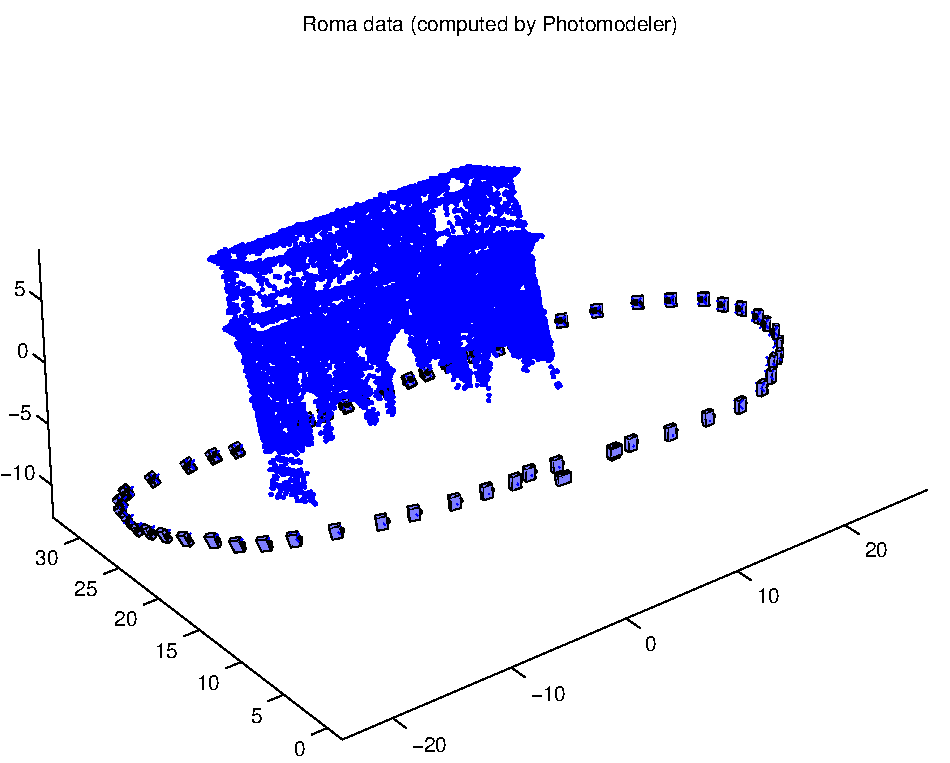
\includegraphics[width=0.6\textwidth]{./ill/roma.pdf}
\caption{\label{fig:roma}
The figure generated by the \texttt{loadplotdemo} demo.}
\end{figure*}

\begin{figure*}[tbp]
\centering
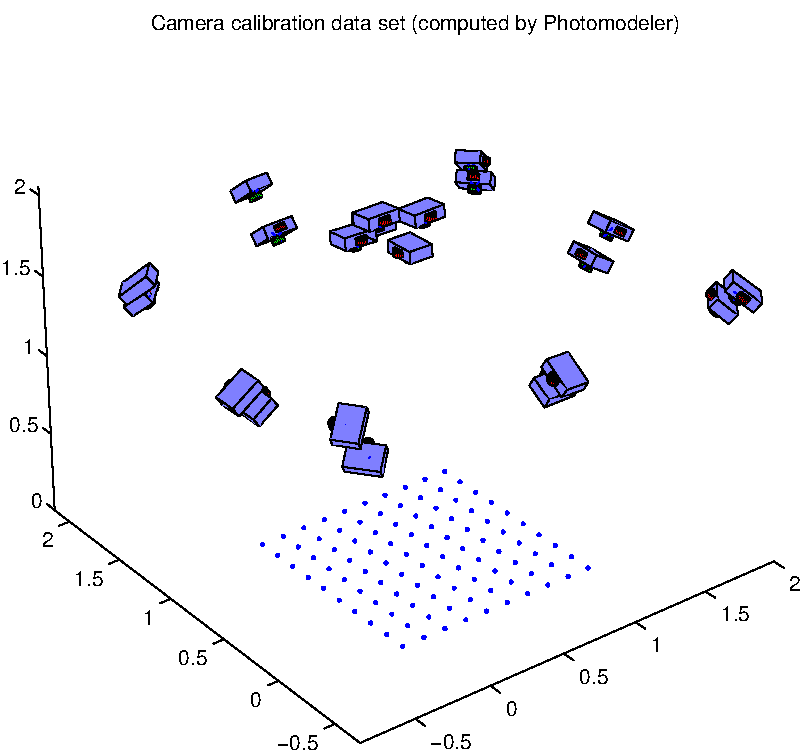
\includegraphics[width=0.6\textwidth]{./ill/ccam.pdf}
\caption{\label{fig:camcalib}
The figure generated by the \texttt{loadplotdemo('cam')} demo.}
\end{figure*}

\subsubsection{Camera calibration}
\label{sec:org8e068b6}

The \texttt{camcaldemo} demo loads the camera calibration export file from
Section~\ref{sec:camcaldata} and runs a camera calibration. The
EXIF focal length is used as the initial value. The other values are
set to ``default'' values, e.g., the principal point at the center of
the sensor and all lens distortion parameters equal to zero. The
initial value for the EO parameters are computed by spatial
resection~\citep[Chap.~11.1.3.4]{Haralick1994:Review,McGlone2004:Manual}
using the control points defined for the PhotoModeler calibration
sheet. The initial OP coordinates are subsequently computed by forward
intersection.

The bundle adjustment is run with Gauss-Newton-Armijo damping
\citep{Borlin2013:Bundle}. The result is given in a number of plot
windows and a Photo-modeler-style result text file. The result plots
are of two kinds: Plots that show the evolution of the iterations and
plots that show the quality of the input or output data. The former
plots may be useful to understand how the bundle adjustment works but
also to ``debug'' a difficult network that has convergence
difficulties. The latter plots give information about the quality of
the result and may also provide clues on how to improve a network when
the bundle did converge.

\paragraph{Evolution plots}
\label{sec:org7948fa9}

\begin{figure}[tbp]
\centering
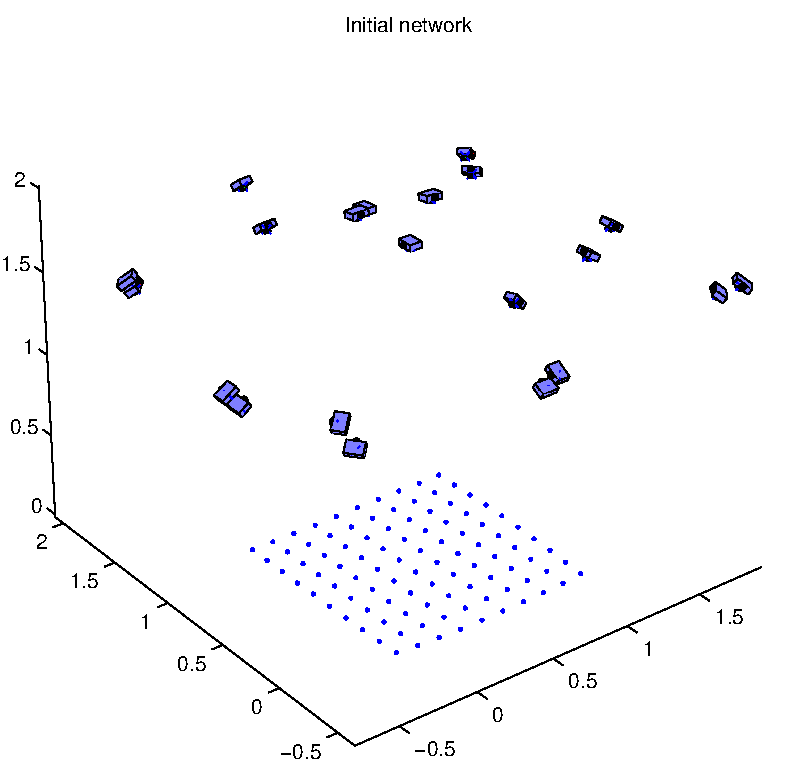
\includegraphics[width=0.6\textwidth]{./ill/ccamx0.pdf}
\caption{\label{fig:camx0}
Initial network configuration for the 3D network. Only the EO and OP parameters are illustrated.}
\end{figure}

\begin{figure}[tbp]
\centering
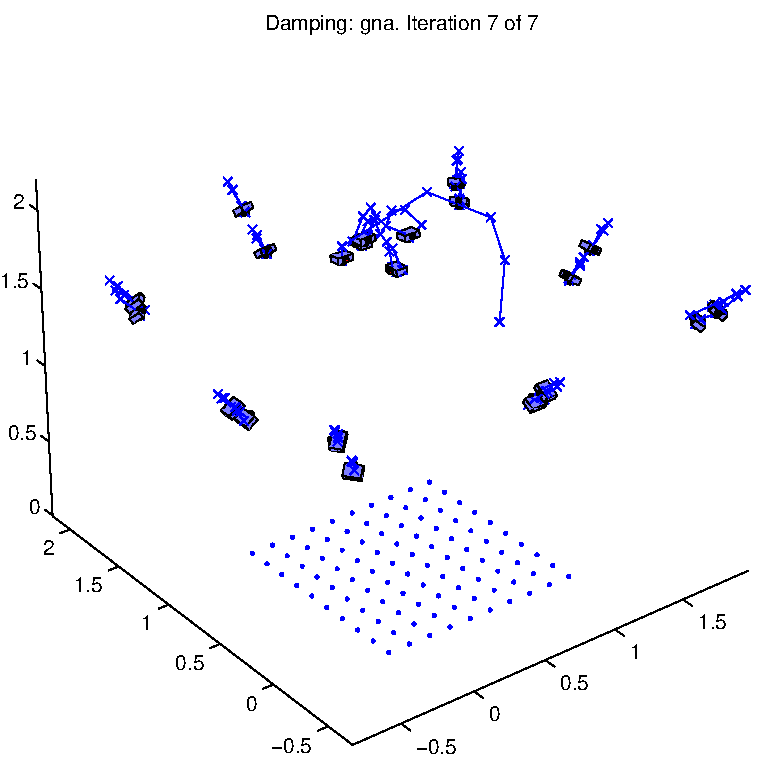
\includegraphics[width=0.6\textwidth]{./ill/ccamxfinal.pdf}
\caption{\label{fig:camxfinal}
Network configuration after convergence, with camera center trace lines. In this example, the variation of the OP coordinates is barely visible.}
\end{figure}

The evolution plots are collected in
figures~\ref{fig:camx0}--\ref{fig:gnatrace}.
Figures~\ref{fig:camx0}--\ref{fig:camxfinal} shows a snapshot of the 3D trace
figure at the beginning and end of the iterations. As default, the
evolution is presented iteration by iteration with intervening presses
of the return key. The figure window is interactive and may be
rotated, zoomed, etc. In this example, it is clear in
Figure~\ref{fig:camxfinal} that one camera station had poorer initial
values than the rest.

\begin{figure}[tbp]
\centering
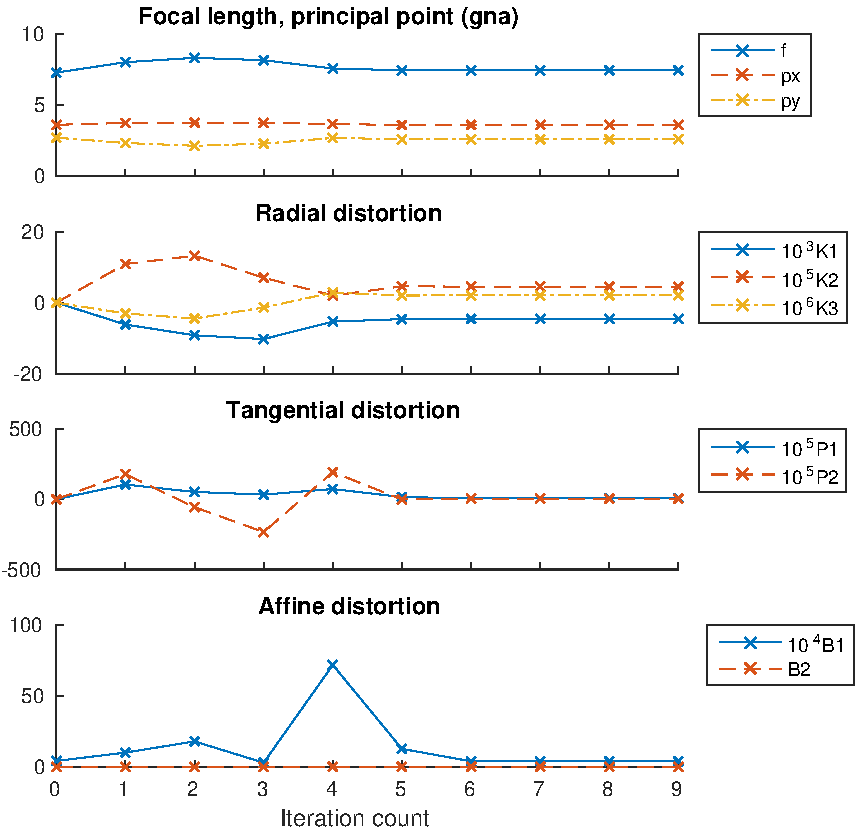
\includegraphics[width=0.6\textwidth]{./ill/ccamiotrace.pdf}
\caption{\label{fig:IOtrace}
Evolution of IO parameters during the iteration sequence.}
\end{figure}

\begin{figure}[tbp]
\centering
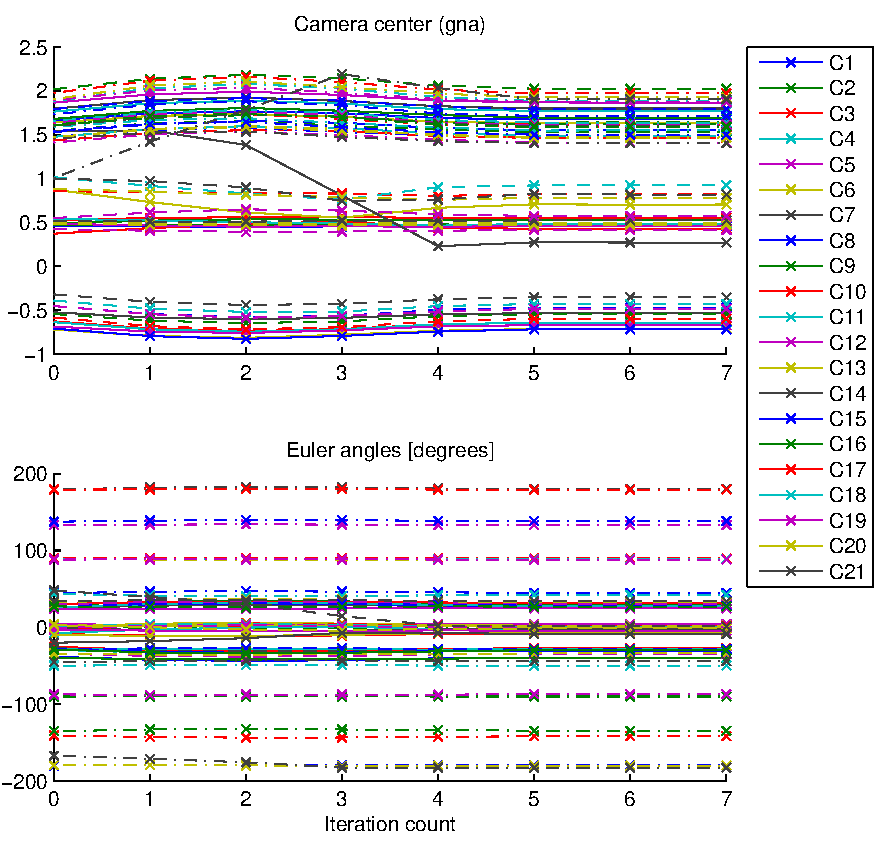
\includegraphics[width=0.6\textwidth]{./ill/ccameotrace.pdf}
\caption{\label{fig:EOtrace}
Evolution of EO parameters during the iteration sequence.}
\end{figure}

\begin{figure}[tbp]
\centering
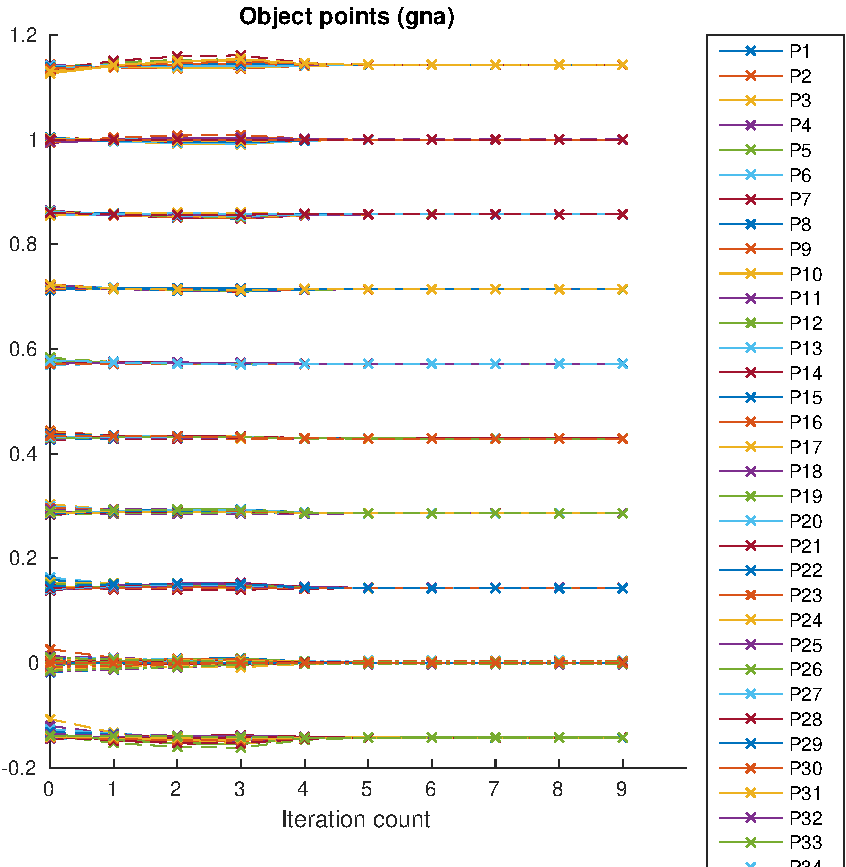
\includegraphics[width=0.6\textwidth]{./ill/ccamoptrace.pdf}
\caption{\label{fig:OPtrace}
Evolution of OP parameters during the iteration sequence.}
\end{figure}

Figures~\ref{fig:IOtrace}--\ref{fig:OPtrace} contain three plots showing the
evolution of the internal orientation (IO), external orientation (EO),
and object point (OP), respectively, during the iterations. The IO
plot is split into a focal/principal point panel and a radial and
tangential distortion panel, where the radial distortion parameters
are scaled to provide more information. The EO plot contains a camera
center panel and an \(\omega\)-\(\phi\)-\(\kappa\) Euler angle panel. The EO and
OP plots are interactive. Lines in the plots or legends may be
selected and all corresponding lines will be highlighted. In the top
panel of Figure~\ref{fig:EOtrace}, the motion of one camera stands out.
Clicking that line reveals that it belongs to camera station~21,
which can be further investigated to decide if it should be excluded
from the calibration.

\begin{figure}[tbp]
\centering
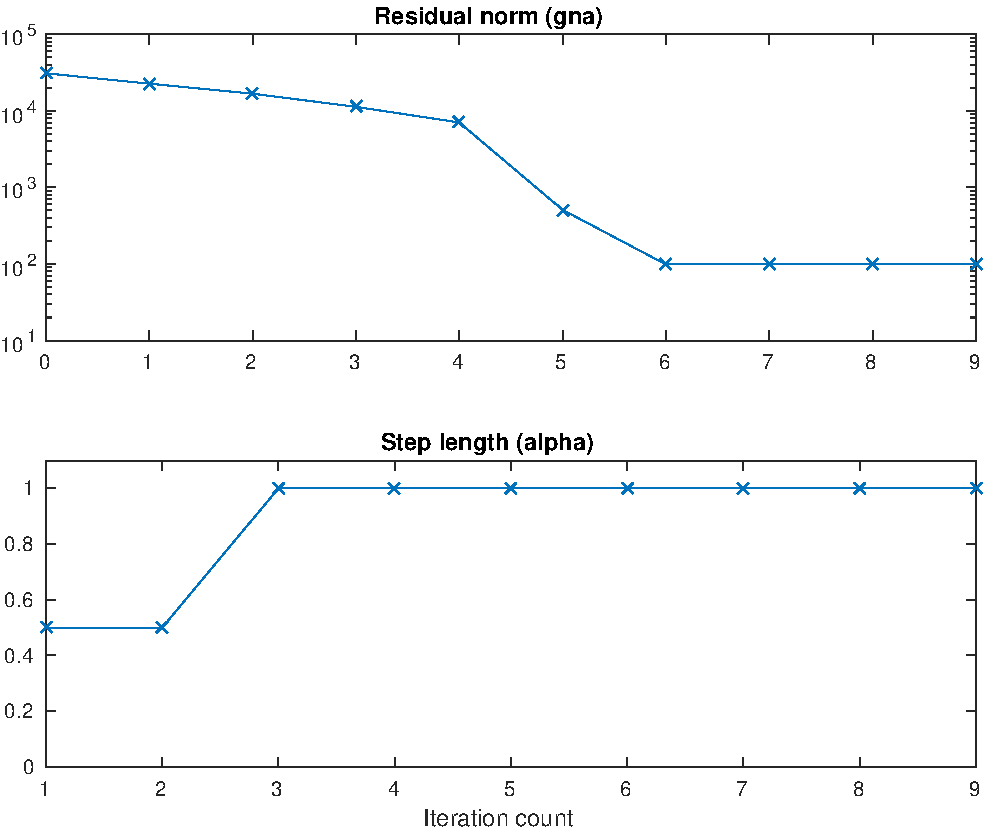
\includegraphics[width=0.6\textwidth]{./ill/ccamgnatrace.pdf}
\caption{\label{fig:gnatrace}
Residual evolution and damping behaviour during the iterations.}
\end{figure}

The final evolution plot, shown in Figure~\ref{fig:gnatrace},
illustrates the evolution of the norm of the total residual and the
damping behaviour, if any, during the bundle iterations. In this
example, the Gauss-Newton-Armijo linesearch damping is active during
the first two iterations. For further details on the damping,
see~\citet{Borlin2013:Bundle}.

\paragraph{Quality plots}
\label{sec:org19bf405}

\begin{figure}[tbp]
\centering
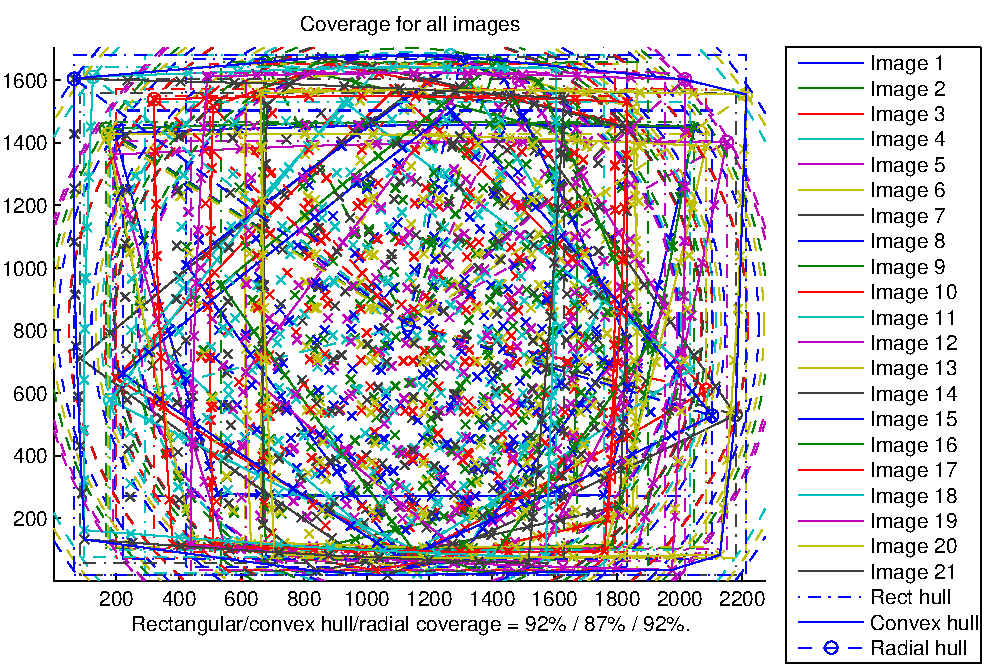
\includegraphics[width=0.6\textwidth]{./ill/ccamcoverage.pdf}
\caption{\label{fig:ccamCoverage}
Plots of input/output statistics: Image coverage.}
\end{figure}

\begin{figure}[tbp]
\centering
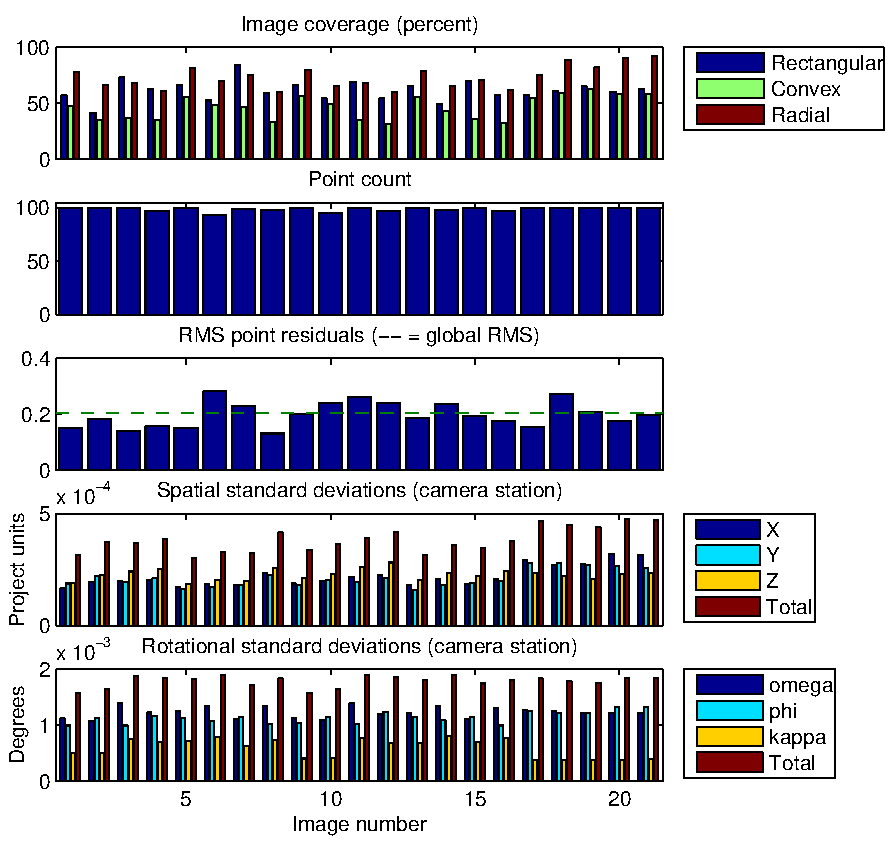
\includegraphics[width=0.6\textwidth]{./ill/ccamimstats.pdf}
\caption{\label{fig:ccamImstats}
Plots of input/output statistics: Image statistics.}
\end{figure}

\begin{figure}[tbp]
\centering
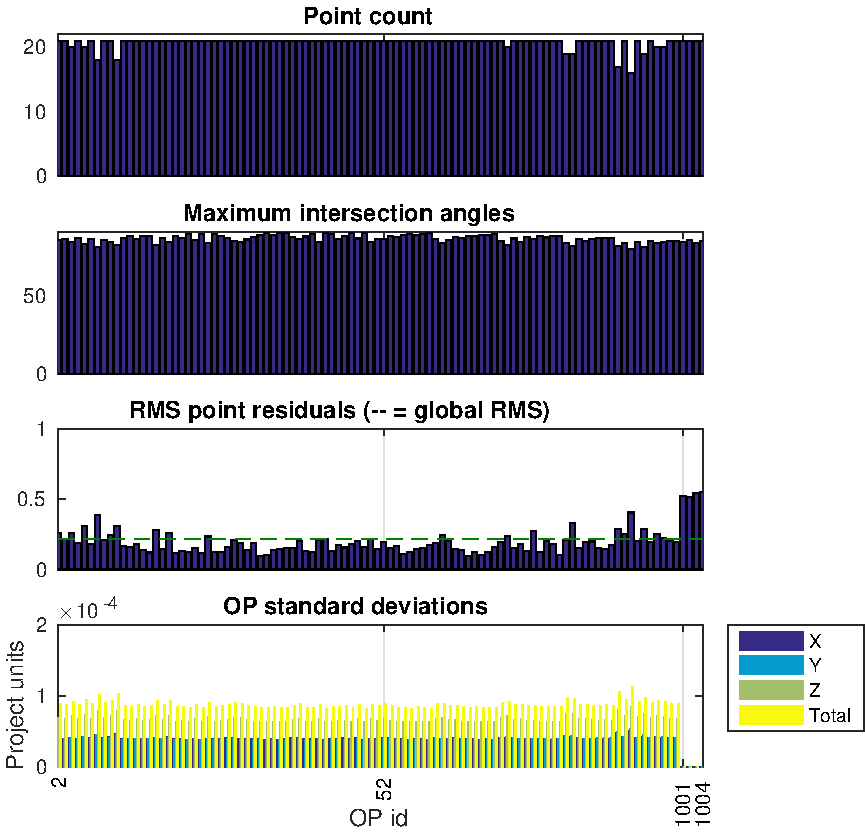
\includegraphics[width=0.6\textwidth]{./ill/ccamopstats.pdf}
\caption{\label{fig:ccamOPstats}
Plots of input/output statistics: Object point statistics.}
\end{figure}

The quality plots are gathered in
figures~\ref{fig:ccamCoverage}--\ref{fig:ccamOPstats}. Per-image quality
statistics is shown in Figure~\ref{fig:ccamImstats}. The statistics
presented for each image are the image coverage (rectangular coverage,
convex hull coverage, and radial coverage); the number of measured
points; the average (RMS) point residual; and the standard deviations
for the EO parameters for the camera stations. In this example, the
data does not give any obvious support to exclude the suspected
image~21 from the calibration.

The image coverage is detailed in a separate
Figure~\ref{fig:ccamCoverage}. The plotted data is selectable. All
observations from a specific image, including their convex hull, will
be highlighted when a point or line is selected.

Finally, the per-OP quality statistics in Figure~\ref{fig:ccamOPstats}
show the number of observations per OP; the maximum ray intersection
angle; the average (RMS) point residual; and the OP coordinate
standard deviation. The presentation may be zoomed to show only a
subset of the OPs by activating the ``zoom'' function of the figure
window.

\paragraph{Result file}
\label{sec:org744b85d}

The result file is modelled after the PhotoModeler result file. The
result file of a successful run is listed in
Appendix~\ref{sec:resultFile}.

\subsubsection{Lens distortion models}
\label{sec:orgf464ab6}

The \texttt{camcaldemo\_allmodels} demo calibrates the camera using
each of the available lens distortion models. A result file is
generate for each model.

\subsubsection{Bundle adjustment}
\label{sec:org224d4a8}

\paragraph{\texttt{Roma}}
\label{sec:orged9028f}
\sloppy The \texttt{romabundledemo} function loads the project from
Section~\ref{sec:loadplotdemo} and present essentially the same plots and
the \texttt{camcaldemo}. This demo uses the PhotoModeler file as input
to the bundle adjustment that runs a few iterations until convergence.
The same result file and result plots as \texttt{camcaldemo} are
essentially generated. Since the project is larger (60 cams/26~000
points) than the previous example (20 cams/100 points), the
computation will take a bit longer. Computation time was around one
minute running on a HP compaq dc7800 with an Intel Core2 Quad CPU
Q9300 @ 2.50GHz under 64-bit Ubuntu 12.04 (kernel 3.5.0-45). Two
variants with self-calibration (\texttt{romabundledemo\_selfcal}) and
image-variant self-calibration (\texttt{romabundledemo\_imagevariant})
are also included. In the latter, the principal point is image-variant
whereas the other IO parameters are block-invariant.

\paragraph{\texttt{Prague'16}}
\label{sec:org740a664}
The \texttt{prague2016\_pm} function displays six projects that
compare the result of the bundle adjustment procedure in DBAT and the
results of PhotoModeler \citep{Borlin2016:External}. Similarily, the
\texttt{prague2016\_ps} function displays the results of a comparison
between DBAT and PhotoScan.

The v0.5.1.6 release includes a fix to a bug the distributed the image
observation weights incorrectly. The result is slightly different
estimation results than in \citet{Borlin2016:External}. However, the
conclusions remain valid.

\paragraph{\texttt{Hamburg'17}}
\label{sec:org06f15c3}
The \texttt{stpierrebundledemo\_ps} function runs a self-calibration
bundle on a Photoscan project included in the StPierre data set.

\paragraph{\texttt{Prior camera observations}}
\label{sec:orgb80f727}
The \texttt{sxb\_prior\_eo} demo shows how to include prior
observations of the camera positions in the bundle.

\subsubsection{Error detection}
\label{sec:orga6db3d1}

Three demos are included to illustrate the error detection
capabilities of \texttt{sprank} (\texttt{dmperm}) and
\texttt{spnrank}. All are modelled from \texttt{camcaldemo}.

\paragraph{Missing observations}
\label{sec:org5f7811e}

The \texttt{camcaldemo\_missing\_obs} demo contains a data file where the image
observations of two object points (id 13 and 60, respectively) have
been deleted. With no observations of either point, the rank
deficiency detected by \texttt{sprank} is six. In the generated result file
(Section~\ref{sec:missingObsResultFile}), the X/Y/Z coordinates
of both points number 12 and 59 (with id 13 and 60, respectively) are
indeed listed as suspicious.

\paragraph{Single-ray observations}
\label{sec:orgcb1e8a2}

The \texttt{camcaldemo\_1ray} demo contains a data file that contains
only one observation of object point with id 88. Since two
observations (one 2D point) is present but three parameter (one 3D
point) is to be estimated, the rank deficiency is one, the rank
deficiency detected by \texttt{sprank} is one. The generated result
file (Section~\ref{sec:singleRayResultFile}) lists one coordinate of
point 87 (with id 88) as suspicious.

\paragraph{Missing datum}
\label{sec:org3dd94bc}

The \texttt{camcaldemo\_no\_datum} demo contains a demo where no datum
has been specified. As in the previous problems, the result is a
numerical problem with a singular (rank deficient) normal matrix.
However, in this case the problem is manifested by that many or all
parameters are linearly dependent of each other. This will not be
detected by \texttt{sprank}. In such a case, the null-space of the
normal matrix will carry information about what parameters are
linearly dependent, i.e. what parameters are part of the problem.
However, when the normal matrix is large, computing the null-space of
the normal matrix in the conventional way using the Matlab function
\texttt{null} will be intractable. Instead, the \texttt{spnrank}
\citep{Foster2009:Calculating} function is used to estimate the rank
deficiency of the normal matrix, i.e. the dimension of the null-space.
Given the dimension of the null-space, a basis for the null-space is
found using Matlab's \texttt{eigs} function. For this demo, the
generated result file (Section~\ref{sec:missingDatumResultFile}) lists
many EO parameters as suspicious. The cause of the problem is less
straight-forward to determine from the list. However, the listed rank
deficiency of seven should be a strong hint of a datum problem.

\begin{sidewaystable}[tbp]
\caption{\label{tab:demos}
Summary of demos.}
\centering
\begin{tabular}{llll}
Demo & Description & Datum & Self-calibration\\
\hline
\texttt{loadplotdemo} & Load and plot & - & -\\
\hline
\texttt{romabundledemo} & Bundle adjustment & Relative dependent orientation & no\\
\texttt{romabundledemo\_selfcal} & Bundle adjustment & Relative dependent orientation & yes\\
\texttt{romabundledemo\_imagevariant} & Bundle adjustment & Relative dependent orientation & split-variant\\
\hline
\texttt{camcaldemo} & Camera calibration & Synthetic control pts & yes\\
\texttt{camcaldemo\_allmodels} & Camera calibration, varying distorion models & Synthetic control pts & yes\\
\texttt{camcaldemo\_missing\_obs} & Exact singular normal matrix & Synthetic control pts & yes\\
\texttt{camcaldemo\_1ray} & Exact singular normal matrix & Synthetic control pts & yes\\
\texttt{camcaldemo\_no\_datum} & Numerically singular normal matrix & Missing & yes\\
\hline
\texttt{prague2016\_pm('c1')} & Camera calibration & Synthetic fixed control points & yes\\
\texttt{prague2016\_pm('c2')} & Camera calibration & Synthetic weighted control points & yes\\
\texttt{prague2016\_pm('s1')} & Bundle adjustment & Fixed ctrl pts from text file & no\\
\texttt{prague2016\_pm('s2')} & Bundle adjustment & Weighted ctrl pts from text file & no\\
\texttt{prague2016\_pm('s4')} & Bundle adjustment & Weighted ctrl pts from text file & no\\
\hline
\texttt{prague2016\_ps('s5')} & Photoscan post-processing & Weighted ctrl pts from psz file & no\\
\hline
\texttt{ps\_postproc('')} & Photoscan post-processing & Weighted ctrl pts from psz file & no\\
\hline
\texttt{stpierrebundledemo\_ps} & Photoscan post-processing & Weighted ctrl pts from psz file & yes\\
\hline
\texttt{sxb\_prior\_eo} & Use of prior camera positions in bundle & Weighted ctrl pts, cam pos from text file & no\\
\hline
\texttt{rundbatdemos} & XML scripts & Varies & varies\\
\end{tabular}
\end{sidewaystable}

\newpage
\subsection{Using your own data}
\label{sec:orgb71a8f9}

\subsubsection{Photoscan/Metashape}
\label{sec:orge838b28}

DBAT can read native Photoscan Archive (\texttt{.psz}) files. DBAT
cannot read Photoscan Project (\texttt{.psx}) files. If you have a
\texttt{.psx} project, use the \emph{Save as\ldots{}} menu in Photoscan and
save the project as a Photoscan Archive (\texttt{.psz}). DBAT has been
tested with Photoscan file versions up to v1.4.0, Photoscan program
version v1.4.4 as well as a pre-release v1.5.0 of Metashape.

The \texttt{ps\_postproc} function can be used to post-process a
Photoscan project. \texttt{loadplotpsz} may be useful to visualize the
project, as computed by Photoscan. As of DBAT version 0.8.5.0, prior
observations of the camera positions are acknowledged and used in the
bundle.

\paragraph{Known limitations}
\label{sec:orgef07f11}

DBAT cannot handle all Photoscan coordinate systems. If you get
strange results, you may have to convert to Local Coordinates.
\texttt{loadplotpsz} may be useful for debugging the input.

\subsubsection{PhotoModeler}
\label{sec:orgfec651d}

This section describes how to import you own data using PhotoModeler
text export files. If you have another type of input file, you may be
able to write your own loader. Otherwise, if you have a text file you
wish to import, feel free to mail the file to the the toolbox authors
and request an import function. Althought we cannot guarantee
anything, we may adhere to the request, time permitting.

\paragraph{Export from PhotoModeler}
\label{sec:org7b431aa}

To import a PhotoModeler project into the toolbox, the following steps
are valid in PhotoModeler Scanner 2012:

\begin{itemize}
\item Export the project using the \emph{Export Text File} menu command. If the
command is not available, follow the instructions in
Appendix~\ref{sec:enableTextExport}.
\item After export, open the \emph{Project/Cameras\ldots{}} dialog and select the
camera that was used in your project.
\item Open the generated text file in a text editor.
\begin{itemize}
\item On the 2nd line (usually reading \texttt{0.00005 20}), append the width
and height in pixels of your images, e.g., to \texttt{0.000500 20 5616
    3744}.
\item Inspect the 4th line. For instance, the original data in
\texttt{roma.txt} was (some trailing zeros removed):

\texttt{24.3581 18.1143 12.0 35.96404 24.0 0.00022 -0.0 0.0 0.0 0.0}

The values correspond to the following camera parameters:

\texttt{focal pp\_x pp\_y format\_w format\_h K1 K2 K3 P1 P2}.

Notice that most of the significant digits of K1--K3 were lost in
the text export.
\item Update the parameter values on the 4th line with values from the
camera dialog \emph{for each parameter with a larger number of
significant digits in the dialog}. This usually means all
parameters except \texttt{format\_w}. In the \texttt{roma.txt} test case, the 4th
line was modified to:

\texttt{24.3581 18.1143 12 35.96404 24 2.174e-4 -1.518e-7 0 0 0}.
\end{itemize}
\end{itemize}

\paragraph{Loading into Matlab}
\label{sec:org3002222}

\begin{itemize}
\item In Matlab, run steps 1.1-1.2 under \texttt{TESTING THE INSTALLATION} from
Section~\ref{sec:install} if not already done.
\item Call \texttt{loadplotdemo} with the name of your text export file as first
parameter. A figure with your camera network, aligned with the first
camera and rotated to have +Z 'up', should now have been generated.
\end{itemize}

\paragraph{Using the bundle adjustment of DBAT}
\label{sec:orgbb57d53}

Modify either of the demo functions or the demo XML files to match
what you want to do. The interesting results may either be in the
plots or in the result file.

\subsection{XML scripts}
\label{sec:xml}
The XML scripting language allow the user to use most of the features
of DBAT without writing or modifying any Matlab code. The processing
is controlled via scripts written in the XML language.
\subsubsection{The XML language}
\label{sec:orgdc559f0}
The XML (eXtensible Markup Language) language \footnote{\url{https://en.wikipedia.org/wiki/XML}} is a structured,
text-based, markup language. The data components are called \emph{elements}
that contain \emph{content} delineated by \emph{tags}. Elements may have
\emph{attributes} that consist of name-value pairs within the opening tag.
For instance, the element
\begin{minted}[autogobble,fontsize=\tiny,frame=single,fontsize=\small]{xml}
<operation min_rays="2">check_ray_count</operation>
\end{minted}
has the content \texttt{check\_ray\_count}, is surrounded by the tag
\texttt{operation} and has an argument named \texttt{min\_rays} with a value of \texttt{2}.
In DBAT, the argument \texttt{min\_rays} with value \texttt{2} will be passed on to
the operation \texttt{check\_ray\_count}. 

The content of one element may be one or more other elements. Thus,
elements may be grouped recursively. For instance, in
\begin{minted}[autogobble,fontsize=\tiny,frame=single,fontsize=\small]{xml}
<operations>
  <operation>spatial_resection</operation>
  <operation>forward_intersection</operation>
  <operation>bundle_adjustment</operation>
</operations>
\end{minted}
the element \texttt{operations} contain three elements \texttt{operation}, that have
the content \texttt{spatial\_resection}, \texttt{forward\_intersection}, and
\texttt{bundle\_adjustment}, respectively. This is used in DBAT XML files to
organize group similar elements together.

\subsubsection{The DBAT XML file}
\label{sec:org9d069c1}

The DBAT function \texttt{rundbatscript} processes a main XML script. The
script is organized into four major parts: metadata, input,
processing, and output.

\paragraph{XML comments}
\label{sec:org2e3a8e4}
The XML language supports comments on the form
\begin{minted}[autogobble,fontsize=\tiny,frame=single,fontsize=\small]{xml}
<!-- Your comment goes here. -->
\end{minted}
As of Matlab Version: 9.4.0.813654 (R2018a), the Matlab XML parser (or
rather, the Java XML parser used by Matlab), has a bug in the comment
parser. As a workaround, surround comments with the \texttt{<c>} tag instead,
as in
\begin{minted}[autogobble,fontsize=\tiny,frame=single,fontsize=\small]{xml}
<c>
  Your comment goes here.
</c>
\end{minted}
\paragraph{Metadata}
\label{sec:org5b7b894}
The metadata section has the tag \texttt{<meta>}. As the name suggests, it is
intended to be used for project metadata. However, the data is not
processed by DBAT and any data may be stored there. Thus, the metadata
section can be extended with any tag. Since the XML language is
standardized, other software may interact with the DBAT XML files for
e.g. storage or searching.

\begin{minted}[autogobble,fontsize=\tiny,frame=single,fontsize=\small]{xml}
<meta>
  <name>Camcaldemo</name>
  <date>2019-10-23</date>
  <author>Niclas Börlin</author>
  <version>1.0</version>
  <project>DBAT</project>
  <project_unit>m</project_unit>
  <purpose>
    Demonstrate camera calibration using the scripting feature of
    DBAT. See also camcaldemo.m in the demo folder.
  </purpose>
  ...
</meta>
\end{minted}

For more examples of metadata blocks, see the example scripts in
Appendix~\ref{sec:XMLdemoScripts}.
\paragraph{Input}
\label{sec:org043e111}
The input section uses the \texttt{<input>} tag and specifies what data to
use for the processing, including camera specifications, control
information, other prior observations, image lists and image
observations. The camera information, image list and image
observations are mandatory. Some information may be stored in separate
XML or text files. See Section~\ref{sec:fileOrganisation} for a
discussion of path names. For a general discussion on text file
formats, see Section~\ref{sec:textFormat}.

\begin{description}
\item[{Cameras}] The camera section uses the \texttt{<cameras>} tag. The camera
information may be specified directly in the main XML
file, as in
\begin{minted}[autogobble,fontsize=\tiny,frame=single,fontsize=\small]{xml}
<cameras>
  <camera>
    <c>Camera specification goes here</c>
  </camera>
  <camera>
    <c>Another specification goes here</c>
  </camera>
</cameras>
\end{minted}
or in a separate camera file, as in
\begin{minted}[autogobble,fontsize=\tiny,frame=single,fontsize=\small]{xml}
<cameras>
  <file>cameras/camera.xml</file>
</cameras>
\end{minted}
For a list of all camera parameters, consult
Appendix~\ref{sec:camSpec}. For an example of a camera file, see
Appendix~\ref{sec:camFileExample}.
\item[{Control points}] The control point section uses the \texttt{<ctrl\_pts>}
tag. Control points are stored in
''comma-separated'' text files. The parsing of the
text files are controlled via a \texttt{format}
attribute. Furthermore, the control points may be
filtered to remove unused control points or points
used as check points. In the example below, the
control points with id 351 and 410 are removed
from the control point list. For a full list of
the supported format components, see
Appendix~\ref{sec:ctrlFormat}. For an example
control point file, see
Appendix~\ref{sec:ctrlExample}.
\begin{minted}[autogobble,fontsize=\tiny,frame=single,fontsize=\small]{xml}
<ctrl_pts>
  <file format="id,label,x,y,z,sx,sy,sz">
    reference/sxb-control.txt
  </file>
  <filter id="351,410">remove</filter>
</ctrl_pts>
\end{minted}
\item[{Check points}] The check point section uses the \texttt{<check\_pts>} tag
and uses the same format as the control point
section. If any point is used as both control and
check point, an error is signalled. In the example
below, the points excluded as control points above
are used as check points.
\begin{minted}[autogobble,fontsize=\tiny,frame=single,fontsize=\small]{xml}
<check_pts>
  <file format="id,label,x,y,z,sx,sy,sz">
    reference/sxb-control.txt
  </file>
  <filter id="351,410">keep</filter>
</check_pts>
\end{minted}
\item[{Images}] The image list section uses the \texttt{<images>} tag. The
information is stored in a comma-separated text file. The
supported format components are listed in
Appendix~\ref{sec:imageFormat}. For an example image list
file, see Appendix~\ref{sec:imageExample}. In the example
below, any relative path name in the \texttt{images.txt} file is
relative to the DBAT installation directory (see
Section~\ref{sec:fileOrganisation}).
\begin{minted}[autogobble,fontsize=\tiny,frame=single,fontsize=\small]{xml}
<images image_base_dir="$DBAT">
  <file format="id,path">images/images.txt</file>
</images>
\end{minted}
The image files are not needed for DBAT computations.
Thus, a non-present image file will only trigger an error
if the image is needed for plotting of, e.g., image
observations.
\item[{Prior EO observations}] The prior EO observations section uses the
\texttt{<prior\_eo>} tag. The data is stored in a comma-separated text
file. In addition to the camera position, camera angles can be
specified, in which case angle units must be specified. The
supported format components are listed in
Appendix~\ref{sec:eoFormat}. An example EO file is presented in
see Appendix~\ref{sec:eoExample}.
\begin{minted}[autogobble,fontsize=\tiny,frame=single,fontsize=\small]{xml}
<prior_eo>
  <file format="id,x,y,z,omega,phi,kappa" units="degrees">
    prior/initial_eo.txt
  </file>
</prior_eo>
\end{minted}
Prior EO observations may be used as prior observations and/or as
initial values for the bundle.
\item[{Image observations}] The image observations section uses the
\texttt{<image\_pts>} tag. The image observations are stored in
comma-separated text files. Multiple files may be specified, as
in the example below. The standard deviations may be read from
the text files or specified via attributes to the \texttt{file} tag. The
supported format components are listed in
Appendix~\ref{sec:imagePtsFormat}.
\begin{minted}[autogobble,fontsize=\tiny,frame=single,fontsize=\small]{xml}
<image_pts>
  <file format="id,im,x,y" sxy="0.5">
    measurements/markpts.txt
  </file>
  <file format="id,im,x,y" sxy="1.0">
    measurements/smartpts.txt
  </file>
</image_pts>
\end{minted}
\end{description}
\paragraph{Processing}
\label{sec:orga178e73}

The processing section uses a single \texttt{<operations>} tag containing one
or more \texttt{<operation>} tags. The listed operations will be executed in
sequence. The operations are of seven types: Sanity checks, filtering,
set initial values, specify parameters to estimate, set the datum,
pre-bundle computation, and execute the bundle proper.

\begin{description}
\item[{Sanity checks}] The sanity check operations include:
\begin{itemize}
\item Check ray count. Verify that no object point has too few rays. The
minimum number of rays is specified via an attribute, as in
\begin{minted}[autogobble,fontsize=\tiny,frame=single,fontsize=\small]{xml}
<operation min_rays="2">check_ray_count</operation>
\end{minted}
An error will be thrown if an object point has fewer than the
specified number of rays. A control point may have one fewer ray
without triggering an error.
\item Future sanity checks include check ray angles, check object point
projections, check structural rank and check numerical rank.
\end{itemize}
\item[{Filtering}] Future filtering operations include:
\begin{itemize}
\item Filter on ray count. Remove any object points
and associated image observations that have too few rays.
\item Filter on intersection angle. Remove any object points that have
too low intersection angle. For this filtering to be applied,
camera and object point positions must have been estimated.
\end{itemize}
\item[{Specify parameters to estimate}] The \texttt{<set\_bundle\_estimate\_params>}
section specifies what parameters should be estimated by the
bundle. The section is structured into IO, EO, and OP
subsections. Within each subsection, the specifications are
parsed in sequence. In the example below, all EO and OP
parameters are estimated, as are all camera parameters except
skew. See Appendix~\ref{sec:setBundleEstimateParams} for a
complete specification of the section.
\begin{minted}[autogobble,fontsize=\tiny,frame=single,fontsize=\small]{xml}
<set_bundle_estimate_params>
  <io>
    <all>true</all>
    <skew>false</skew>
  </io>
  <eo>true</eo>
  <op>true</op>
</set_bundle_estimate_params>
\end{minted}
\item[{Set initial values}] The \texttt{<set\_initial\_values>} operation specifies
initial values for the bundle. This should be used if the initial
values are not computed by other means, e.g., by spatial
intersection or forward intersection. Often, the initial values
may be set to values loaded in the \texttt{input} section. In the
example below, the IO and OP parameters are set to their
pre-loaded values. No values are specified for the EO parameters,
and they must be estimated by, e.g., spatial intersection. See
Appendix~\ref{sec:setInitialValues} for a complete specification.
\begin{minted}[autogobble,fontsize=\tiny,frame=single,fontsize=\small]{xml}
<set_initial_values>
  <io>loaded</io>
  <op>loaded</op>
</set_initial_values>
\end{minted}
\item[{Set datum}] Usually, the datum is set via control points. For a
control-point-free project, it is possible to set up
the project for dependent relative orientation instead.
In that case, the EO parameters of one camera is fixed
together with a position coordinate of another camera.
In the example below, camera number 1 is used as the
reference camera. The coordinate of the second camera
is set to make the baseline as long as possible. If the
baseline parameter is \texttt{x}, \texttt{y}, or \texttt{z}, the coordinate
selection for the second camera is restricted to that
coordinate.
\begin{minted}[autogobble,fontsize=\tiny,frame=single,fontsize=\small]{xml}
<operation>
  <set_datum ref_cam="1" ref_base="longest">depend</set_datum>
</operation>
\end{minted}
\item[{Pre-bundle computations}] The pre-bundle computations include
\begin{description}
\item[{Spatial resection}] Estimate external orientation parameters by
spatial resection. The operation will fail if IO parameters are
unset or too few control points are visible in some image.
\begin{minted}[autogobble,fontsize=\tiny,frame=single,fontsize=\small]{xml}
<operation>spatial_resection</operation>
\end{minted}
\item[{Forward intersection}] Compute OP coordinates using forward
intersection. Only the object points that are to be estimated
by the bundle are computed. The operation will fail unless the
IO and EO parameters are set and that at least two image points
are present for every object point.
\begin{minted}[autogobble,fontsize=\tiny,frame=single,fontsize=\small]{xml}
<operation>forward_intersection</operation>
\end{minted}
\end{description}
\item[{The bundle proper}] Execute the bundle adjustment procedure. All
parameters must have initial values and the parameters to
estimate must have been set.
\begin{minted}[autogobble,fontsize=\tiny,frame=single,fontsize=\small]{xml}
<operation>bundle_adjustment</operation>
\end{minted}
\end{description}
\paragraph{Output}
\label{sec:orgf998710}
The output section specifies what plots (\texttt{<plots>}) and files
(\texttt{<files>}) should be produced after the completion of the processing.
A complete list of the plots that can be produced is given in
Appendix~\ref{sec:plots}. A list of the output files that can be
generated is presented in Appendix~\ref{sec:outputFiles}.
\paragraph{File organisation}
\label{sec:fileOrganisation}
\sloppy
The \texttt{<input>} and output \texttt{<files>} tags support the attribute
\texttt{base\_dir} that is used to simplify the organisation of files that
belong to the same project. If the \texttt{base\_dir} attribute is specified,
any relative path name \footnote{Path names can be absolute or relative. An absolute
path name starts with a root symbol (backslash \texttt{\textbackslash{}} on Windows, slash
\texttt{/} on other operating systems) or or a drive letter followed by a
colon, e.g. \texttt{C:\textbackslash{}}. A relative path starts with something else.} in the subblock is assumed to
be rooted in \texttt{base\_dir}. For instance, the block
\begin{minted}[autogobble,fontsize=\tiny,frame=single,fontsize=\small]{xml}
<input base_dir="C:/projects/sxb">
  ...
  <ctrl_pts>
    <file format="id,label,x,y,z,sx,sy,sz">
      reference/sxb-control.txt
    </file>
  </ctrl_pts>
  ...
</input>
\end{minted}
will load the control points from the file
\texttt{C:/projects/sxb/reference/sxb-control.txt}. The \texttt{base\_dir} attribute
can be any path. Furthermore, \texttt{base\_dir} can be specified to be
relative to the special directories listed below.

\sloppy
\begin{description}
\item[{\texttt{\$DBAT}}] The root of the DBAT installation, i.e., the directory
that contains the \texttt{README.txt} file.
\item[{\texttt{\$HOME}}] The home directory of the user, as known to Matlab via
the \texttt{user.home} Java property \footnote{The Matlab command is
\texttt{char(java.lang.System.getProperty('user.home'))}.}. This
is typically \texttt{C:\textbackslash{}Users\textbackslash{}username} on Windows,
\texttt{/Users/username} on Mac/OS X, and \texttt{/home/username} on
Linux, where 'username' is the current user name.
\item[{\texttt{\$HERE}}] The directory containing the XML file in use.
\end{description}

\sloppy
Furthermore, the \texttt{images} tag supports another tag \texttt{image\_base\_dir}
that can be used to specify a root directory for the images. For instance,
the block
\begin{minted}[autogobble,fontsize=\tiny,frame=single,fontsize=\small]{xml}
<input base_dir="C:/projects/sxb">
  ...
  <images image_base_dir="Z:/server/project_images/sxb">
    <file format="id,path">images/images.txt</file>
  </images>
  ...
</input>
\end{minted}
specifies that any relative path name loaded from \texttt{images.txt} is
relative to the path \texttt{Z:/server/project\_images/sxb}. Note that the
path \texttt{images/images.txt} is relative to the input \texttt{base\_dir}, i.e.,
the full path name is \texttt{C:/projects/sxb/images/images.txt}.

\paragraph{Text files and format strings}
\label{sec:textFormat}
Several types of data is stored in ''comma-separated'' text files.
DBAT uses format strings to indicate what data is to be read or
written to each file. As default, the text files may include comment
lines starting with the hash (\texttt{\#}) character. The non-comment lines
contain the specified information, separated by commas \footnote{The DBAT back-end supports other separators and comment
characters. This support is not yet implemented in the DBAT front-end
XML parser.}. The
elements of the format are numeric or strings. Please note that any
string cannot contain the separator character, i.e. a comma.

To avoid processing incorrect data, DBAT will require that each data
line conforms to the format. If too few or too many elements are
present on a data line, DBAT will signal an error. To allow some
flexibility of what data to use, the format keyword \texttt{ignored} may be
used to indicate that a data item is present, but should be ignored.
For instance, if the data stored in a control point file corresponds
to the format \texttt{"id,label,x,y,z,sx,sy,sz"}, but the standard deviations
should be ignored, the format string
\texttt{"id,label,x,y,z,ignored,ignored,ignored"} should be used.

\subsubsection{Example scripts}
\label{sec:org8fe4e31}

\sloppy 
The supplied scripts are presented in
Appendix~\ref{sec:XMLdemoScripts}. To run one of the supplied scripts,
call \texttt{rundbatscript} with either of the strings \texttt{camcaldemo},
\texttt{romabundledemo}, or \texttt{sxb} as arguments. If you wish to locate a
script yourself, start \texttt{rundbatscript} without any argument and you
will be asked about the location of the script to run.

\newpage

\section{References}
\label{sec:org0b14303}

\bibliography{ref}

\newpage
\appendix

\section{License}
\label{sec:license}
\begin{minted}[autogobble,fontsize=\tiny,frame=single]{text}
# == LICENSE ==
#
# Copyright (C) 2013-2019, Niclas Börlin, niclas.borlin@cs.umu.se (*),
# and Pierre Grussenmeyer, pierre.grussenmeyer@insa-strasbourg.fr (**).
# All rights reserved.
#
# (*)  Department of Computing Science, Umeå University, Sweden. 
# (**) ICube Laboratory UMR 7357, Photogrammetry and Geomatics Group,
#      Institut national des sciences appliquées de Strasbourg,
#      Strasbourg, France.  
#
# Redistribution and use in source and binary forms, with or without
# modification, are permitted provided that the following conditions
# are met:
#
# 1. Redistributions of source code must retain the above copyright
#    notice, this list of conditions and the following disclaimer.
#
# 2. Redistributions in binary form must reproduce the above copyright
#    notice, this list of conditions and the following disclaimer in
#    the documentation and/or other materials provided with the
#    distribution.
#
# 3. If you use the code, or derivatives thereof, for scientific
#    publications, you should refer to on or more of the papers in the
#    REFERENCES section.
#
# THIS SOFTWARE IS PROVIDED BY THE COPYRIGHT HOLDERS AND CONTRIBUTORS
# "AS IS" AND ANY EXPRESS OR IMPLIED WARRANTIES, INCLUDING, BUT NOT
# LIMITED TO, THE IMPLIED WARRANTIES OF MERCHANTABILITY AND FITNESS
# FOR A PARTICULAR PURPOSE ARE DISCLAIMED. IN NO EVENT SHALL THE
# COPYRIGHT HOLDER OR CONTRIBUTORS BE LIABLE FOR ANY DIRECT, INDIRECT,
# INCIDENTAL, SPECIAL, EXEMPLARY, OR CONSEQUENTIAL DAMAGES (INCLUDING,
# BUT NOT LIMITED TO, PROCUREMENT OF SUBSTITUTE GOODS OR SERVICES;
# LOSS OF USE, DATA, OR PROFITS; OR BUSINESS INTERRUPTION) HOWEVER
# CAUSED AND ON ANY THEORY OF LIABILITY, WHETHER IN CONTRACT, STRICT
# LIABILITY, OR TORT (INCLUDING NEGLIGENCE OR OTHERWISE) ARISING IN
# ANY WAY OUT OF THE USE OF THIS SOFTWARE, EVEN IF ADVISED OF THE
# POSSIBILITY OF SUCH DAMAGE.
#
#
# == REFERENCES ==
#
# Börlin and Grussenmeyer (2013). "Bundle adjustment with and without
#     damping", Photogrammetric Record, vol. 28(144):396-415.
#     DOI: 10.1111/phor.12037.
# Börlin and Grussenmeyer (2013). "Experiments with Metadata-derived
#     Initial Values and Linesearch Bundle Adjustment in Architectural
#     Photogrammetry", ISPRS Annals of the Photogrammetry, Remote
#     Sensing, and Spatial Information Sciences, vol II-5/W1:43-48.
#     DOI: 10.5194/isprsannals-II-5-W1-43-2013.
# Börlin and Grussenmeyer (2014). "Camera Calibration using the Damped
#     Bundle Adjustment Toolbox", ISPRS Annals of the Photogrammetry,
#     Remote Sensing, and Spatial Information Sciences, vol
#     II-5:89-96. DOI: 10.5194/isprsannals-II-5-89-2014.
# Börlin and Grussenmeyer (2016). "External Verification of the Bundle
#     Adjustment in Photogrammetric Software using the Damped Bundle
#     Adjustment Toolbox", ISPRS Archives XLI-B5, p. 7-14.
#     DOI: 10.5194/isprs-archives-XLI-B5-7-2016.
# Murtiyoso, Grussenmeyer, and Börlin (2017). "Reprocessing close
#     range terrestrial and UAV photogrammetric projects with the DBAT
#     toolbox for independent verification and quality control.",
#     ISPRS Archives XLII-2/W8:171-177.
#     DOI: 10.5194/isprs-archives-XLII-2-W8-171-2017.
# Börlin, Murtiyoso, Grussenmeyer, Menna, and Nocerino (2018).
#     "Modular bundle adjustment for photogrammeric computations",
#     ISPRS Archives XLII-2:133-140.
#     DOI: 10.5194/isprs-archives-XLII-2-133-2018.
# Börlin, Murtiyoso, Grussenmeyer, Menna, and Nocerino (2019).
#     "Flexible Photogrammetric Computations using Modular Bundle Adjustment",
#     Photogrammetric Engineering and Remote Sensing, vol. 85(5):361-369.
#     DOI: 10.14358/PERS.85.5.361.
# Börlin, Murtiyoso, P. Grussenmeyer (2019).
#     "Implementing Functional Modularity for Processing of General
#     Photogrammetric Data with the Damped Bundle Adjustment Toolbox (DBAT)",
#     ISPRS Archives, XLII-2/W17, p. 69-75.
#     DOI: 10.5194/isprs-archives-XLII-2-W17-69-2019.
#
#
\end{minted}

\section{Enabling text export from PhotoModeler}
\label{sec:enableTextExport}
Some versions of PhotoModeler do not have the text file export option
enabled by default. In that case, the following steps worked in
PhotoModeler Scanner 2012:

\begin{itemize}
\item Right-click on the main window toolbar, select \emph{Customize
toolbar\ldots{}}.
\item In the \emph{Commands} tab, select the \emph{File} category.
\item Drag the \emph{Export Text File\ldots{}} command to a toolbar of your choice.
\item Now you should be able to export your project as a text file by
clicking on the \emph{Export Text File} button.
\end{itemize}

\section{Rotation model}
\label{sec:org223ff88}

Currently, the only supported rotation model is the omega-phi-kappa
Euler angle rotation model \citep[Ch. 2.1.2.3]{McGlone2004:Manual}.

\section{Result files}
\label{sec:orga25538a}
\subsection{Result file with missing observations}
\label{sec:missingObsResultFile}
\begin{minted}[autogobble,fontsize=\tiny,frame=single]{text}
Damped Bundle Adjustment Toolbox result file
   Project Name: Bundle Soln PhotoModeler Calibration Project
   Problems and suggestions:
      Project Problems:
         Structural rank: 417 (deficiency: 6)
            DMPERM suggests the following parameters have problems:
               OX-12/13
               OY-12/13
               OZ-12/13
               OX-59/60
               OY-59/60
               OZ-59/60
         Numerical rank: not tested.
      Problems related to the processing: (1)
         Bundle failed with code -4 (see below for details).
.
.
.
\end{minted}

\subsection{Result file with single-ray observations}
\label{sec:singleRayResultFile}
\begin{minted}[autogobble,fontsize=\tiny,frame=single]{text}
Damped Bundle Adjustment Toolbox result file
   Project Name: Bundle Soln PhotoModeler Calibration Project
   Problems and suggestions:
      Project Problems:
         Structural rank: 422 (deficiency: 1)
            DMPERM suggests the following parameters have problems:
               OZ-87/88
         Numerical rank: not tested.
      Problems related to the processing: (1)
         Bundle failed with code -4 (see below for details).
.
.
.
\end{minted}

\subsection{Result file with missing datum}
\label{sec:missingDatumResultFile}
\begin{minted}[autogobble,fontsize=\tiny,frame=single]{text}
Damped Bundle Adjustment Toolbox result file
   Project Name: Bundle Soln PhotoModeler Calibration Project
   Problems and suggestions:
      Project Problems:
         Structural rank: ok.
         Numerical rank: 428 (deficiency: 7)
            Null-space suggest the following parameters are part of the problem:
               Vector 1 (eigenvalue 1.36254e-18):
                  (EX-21, -0.156)
                  (EX-9, -0.13)
                  (EX-13, -0.12)
                  (EX-10, -0.119)
                  (EX-11, -0.115)
                  (EX-12, -0.108)
                  (EX-14, -0.104)
               Vector 2 (eigenvalue -1.60532e-17):
                  (EX-21, 0.207)
                  (EY-21, 0.195)
                  (EY-1, 0.192)
                  (EY-2, 0.178)
                  (EX-13, 0.167)
                  (EY-15, 0.166)
                  (EY-3, 0.166)
                  (EY-4, 0.163)
                  (EY-16, 0.161)
                  (EX-14, 0.157)
                  (EX-15, 0.151)
                  (EX-11, 0.149)
                  (EY-18, 0.147)
                  (EX-12, 0.146)
                  (EX-16, 0.145)
                  (EY-20, 0.133)
                  (EY-17, 0.128)
               Vector 3 (eigenvalue 5.21745e-17):
                  (om-21, -0.16)
                  (EX-3, -0.155)
                  (EX-4, -0.151)
                  (EX-5, -0.147)
                  (EX-6, -0.136)
                  (EZ-7, 0.132)
                  (om-13, -0.129)
                  (EX-1, -0.129)
                  (om-15, -0.127)
                  (om-16, -0.125)
                  (EZ-8, 0.125)
                  (om-14, -0.125)
                  (EZ-9, 0.122)
                  (EX-2, -0.117)
                  (om-11, -0.116)
                  (EZ-10, 0.116)
                  (om-12, -0.114)
                  (om-18, -0.113)
                  (om-20, -0.113)
                  (EZ-11, 0.111)
                  (EX-7, -0.111)
                  (EZ-12, 0.11)
                  (om-19, -0.109)
                  (om-9, -0.108)
                  (EZ-5, 0.107)
                  (om-1, -0.106)
                  (om-17, -0.106)
                  (om-2, -0.105)
                  (om-10, -0.105)
               Vector 4 (eigenvalue -5.5516e-17):
                  (EZ-21, -0.174)
                  (EX-5, -0.13)
                  (EX-7, -0.129)
                  (EX-8, -0.12)
                  (EX-6, -0.119)
                  (EY-9, -0.114)
                  (EY-11, -0.111)
               Vector 5 (eigenvalue -1.45759e-16):
                  (EY-7, 0.158)
                  (EY-5, 0.154)
                  (EY-8, 0.153)
                  (EY-9, 0.151)
                  (om-4, -0.147)
                  (EY-19, 0.147)
                  (om-3, -0.144)
                  (EY-6, 0.143)
                  (EY-10, 0.143)
                  (EY-17, 0.133)
                  (EZ-3, -0.132)
                  (EZ-4, -0.129)
                  (om-17, -0.126)
                  (om-19, -0.126)
                  (om-18, -0.125)
                  (om-1, -0.124)
                  (om-9, -0.124)
                  (om-2, -0.124)
                  (EY-18, 0.121)
                  (om-10, -0.121)
                  (EY-20, 0.12)
                  (om-20, -0.12)
                  (om-5, -0.12)
                  (EZ-2, -0.118)
                  (EZ-1, -0.118)
                  (om-6, -0.116)
                  (ph-9, -0.114)
                  (ph-7, -0.113)
                  (ph-11, -0.112)
                  (EY-11, 0.112)
                  (ph-12, -0.111)
                  (ph-8, -0.11)
                  (ph-10, -0.109)
                  (ph-5, -0.108)
                  (om-11, -0.108)
                  (EY-12, 0.107)
                  (EZ-5, -0.106)
                  (ph-13, -0.106)
                  (om-7, -0.104)
                  (ph-19, -0.104)
                  (om-12, -0.104)
                  (ph-14, -0.104)
               Vector 6 (eigenvalue -1.54875e-16):
                  (om-21, 0.185)
                  (ph-9, -0.174)
                  (EZ-21, 0.174)
                  (ph-10, -0.169)
                  (ph-11, -0.167)
                  (ph-7, -0.167)
                  (ph-8, -0.165)
                  (ph-12, -0.164)
                  (EX-9, -0.152)
                  (EX-7, -0.151)
                  (EX-8, -0.151)
                  (EY-11, -0.148)
                  (EY-12, -0.146)
                  (EX-10, -0.146)
                  (EZ-15, 0.142)
                  (EZ-16, 0.137)
                  (EY-13, -0.136)
                  (ph-5, -0.135)
                  (EY-14, -0.133)
                  (EZ-13, 0.127)
                  (ph-13, -0.127)
                  (EZ-14, 0.126)
                  (ph-14, -0.124)
                  (ph-6, -0.123)
                  (ph-19, -0.12)
                  (EY-21, -0.117)
               Vector 7 (eigenvalue 1.9046e-16):
                  (ph-1, 0.194)
                  (ph-2, 0.194)
                  (ph-15, 0.173)
                  (EX-2, 0.173)
                  (om-5, -0.173)
                  (ph-16, 0.169)
                  (ph-4, 0.169)
                  (EX-1, 0.168)
                  (ph-3, 0.164)
                  (om-8, -0.163)
                  (om-7, -0.16)
                  (om-6, -0.16)
                  (ph-21, 0.157)
                  (EY-21, -0.138)
                  (EY-5, 0.138)
                  (EY-6, 0.132)
                  (om-3, -0.127)
                  (ph-20, 0.126)
                  (om-4, -0.125)
      Problems related to the processing: (1)
         Bundle failed with code -2 (see below for details).
.
.
.
\end{minted}

\newpage
\subsection{Successful result file example}
\label{sec:resultFile}
\begin{minted}[autogobble,fontsize=\tiny,frame=single]{text}
Damped Bundle Adjustment Toolbox result file
   Project
      Name             : Bundle Soln PhotoModeler Calibration Project
      Computation UUID : 08bac37e-33f2-43f2-b581-32df2721bd22
      Input file name  : /home/niclas/dbat/data/dbat/pmexports/camcal-pmexport.txt
      Ctrl pt file     : /home/niclas/dbat/data/dbat/ref/camcal-fixed.txt
   Problems and suggestions:
      Project Problems:
         Structural rank: ok.
         Numerical rank: ok.
      Problems related to the processing: (1)
         One or more of the camera parameter has a high correlation (see below).
   Information from last bundle
      Last Bundle Run:        10-Dec-2019 00:09:11
      DBAT version:           0.9.1.2 (2019-12-09)
      MATLAB version:         9.4.0.813654 (R2018a)
      Host system:            GLNXA64 (endian=L, max #elems=281474976710655)
      Host name:              trillian
      Status:                 OK
      Sigma0:                 1.6148
      Sigma0 (pixels):        0.16148
      Redundancy              3725
      Number of params:       423 (9 IO, 126 EO, 288 OP)
      Number of observations: 4148 (4148 IP, 0 IO, 0 EO, 0 OP)
      Processing options:
         Orientation:             on
         Global optimization:     on
         Calibration:             on
         Constraints:             off
         Maximum # of iterations: 20
         Convergence tolerance:   1e-06
         Termination criteria:    relative
         Singular test:           on
         Chirality veto:          off
         Damping:                 gna
         Camera unit (cu):        mm
         Object space unit (ou):  m
         Initial value comment:   Camera calibration from EXIF value
      Total error:
         Number of stages:     1
         Number of iterations: 9
         First error:          30873.9
         Last error:           98.556
         Execution time (s):   0.74
      Lens distortion models:
         Backward (Photogrammetry) model 3
      Cameras:
         Calibration: yes (cc px py as K1 K2 K3 P1 P2)
         Camera1 (simple)
            Lens distortion model:
               Backward (Photogrammetry) model 3
            Camera Constant:
               Value:        7.457 mm
               Deviation:    0.00105 mm
            px - principal point x:
               Value:        3.61546 mm
               Deviation:    0.00082 mm
            py - principal point y:
               Value:        2.61329 mm
               Deviation:    0.00098 mm
            Format width:
               Value:        7.25301 mm
            Format height:
               Value:        5.43764 mm
            K1 - radial distortion 1:
               Value:        0.00458861 mm^(-3)
               Deviation:    2.21e-05 mm^(-3)
               Significance: p=1.00
               Cumulative significance:p=1.00
            K2 - radial distortion 2:
               Value:        -4.51351e-05 mm^(-5)
               Deviation:    2.65e-06 mm^(-5)
               Significance: p=1.00
               Cumulative significance:p=1.00
               Correlations over 95%: K3:-97.9%.
            K3 - radial distortion 3:
               Value:        -2.05253e-06 mm^(-7)
               Deviation:    1.01e-07 mm^(-7)
               Significance: p=1.00
               Cumulative significance:p=1.00
               Correlations over 95%: K2:-97.9%.
            P1 - decentering distortion 1:
               Value:        -6.12803e-05 mm^(-3)
               Deviation:    3.52e-06 mm^(-3)
               Significance: p=1.00
            P2 - decentering distortion 2:
               Value:        -4.41172e-05 mm^(-3)
               Deviation:    3.94e-06 mm^(-3)
            as - off-unit aspect parameter:
               Value:        0.000389598 
               Deviation:    2.08e-05 
               Significance: p=1.00
            sk - skew:
               Value:        0 
            Image width:
               Value:        2272 px
            Image height:
               Value:        1704 px
            X resolution:
               Value:        313.249 px/mm
            Y resolution:
               Value:        313.371 px/mm
            Pixel width:
               Value:        0.00319235 mm
            Pixel height:
               Value:        0.0031911 mm
         Rated angle of view (h,v,d): (52, 40, 63) deg
         Largest distortion: 0.37 mm (116.2 px, 8.2% of half-diagonal)
      Precisions / Standard Deviations:
         Photograph Standard Deviations:
            Photo 1: P8250021.JPG
               Omega:
                  Value:     -39.413082 deg
                  Deviation: 0.0085 deg
               Phi:
                  Value:     -1.183179 deg
                  Deviation: 0.00761 deg
               Kappa:
                  Value:     -179.838467 deg
                  Deviation: 0.00275 deg
               Xc:
                  Value:     0.454947 ou
                  Deviation: 0.000155 ou
               Yc:
                  Value:     1.793849 ou
                  Deviation: 0.000179 ou
               Zc:
                  Value:     1.468066 ou
                  Deviation: 0.000207 ou
            Photo 2: P8250022.JPG
               Omega:
                  Value:     -39.734523 deg
                  Deviation: 0.00816 deg
               Phi:
                  Value:     -1.813688 deg
                  Deviation: 0.00886 deg
               Kappa:
                  Value:     -90.123062 deg
                  Deviation: 0.00289 deg
               Xc:
                  Value:     0.470305 ou
                  Deviation: 0.000186 ou
               Yc:
                  Value:     2.026401 ou
                  Deviation: 0.000219 ou
               Zc:
                  Value:     1.639148 ou
                  Deviation: 0.000232 ou
            Photo 3: P8250023.JPG
               Omega:
                  Value:     -27.227000 deg
                  Deviation: 0.0105 deg
               Phi:
                  Value:     -28.559177 deg
                  Deviation: 0.00753 deg
               Kappa:
                  Value:     -141.839170 deg
                  Deviation: 0.00538 deg
               Xc:
                  Value:     -0.644442 ou
                  Deviation: 0.000188 ou
               Yc:
                  Value:     1.466578 ou
                  Deviation: 0.000179 ou
               Zc:
                  Value:     1.580187 ou
                  Deviation: 0.000243 ou
            Photo 4: P8250024.JPG
               Omega:
                  Value:     -28.556794 deg
                  Deviation: 0.00881 deg
               Phi:
                  Value:     -30.289704 deg
                  Deviation: 0.00923 deg
               Kappa:
                  Value:     -49.786720 deg
                  Deviation: 0.00467 deg
               Xc:
                  Value:     -0.643144 ou
                  Deviation: 0.000198 ou
               Yc:
                  Value:     1.490295 ou
                  Deviation: 0.000202 ou
               Zc:
                  Value:     1.637492 ou
                  Deviation: 0.000246 ou
            Photo 5: P8250025.JPG
               Omega:
                  Value:     4.385418 deg
                  Deviation: 0.00943 deg
               Phi:
                  Value:     -34.659929 deg
                  Deviation: 0.00863 deg
               Kappa:
                  Value:     -87.134063 deg
                  Deviation: 0.00519 deg
               Xc:
                  Value:     -0.671014 ou
                  Deviation: 0.000158 ou
               Yc:
                  Value:     0.417412 ou
                  Deviation: 0.000144 ou
               Zc:
                  Value:     1.409244 ou
                  Deviation: 0.000193 ou
            Photo 6: P8250026.JPG
               Omega:
                  Value:     2.063986 deg
                  Deviation: 0.0103 deg
               Phi:
                  Value:     -33.988460 deg
                  Deviation: 0.00823 deg
               Kappa:
                  Value:     1.485869 deg
                  Deviation: 0.00587 deg
               Xc:
                  Value:     -0.712797 ou
                  Deviation: 0.000177 ou
               Yc:
                  Value:     0.476083 ou
                  Deviation: 0.000155 ou
               Zc:
                  Value:     1.465130 ou
                  Deviation: 0.000203 ou
            Photo 7: P8250027.JPG
               Omega:
                  Value:     27.342174 deg
                  Deviation: 0.00854 deg
               Phi:
                  Value:     -28.292503 deg
                  Deviation: 0.00875 deg
               Kappa:
                  Value:     -44.210389 deg
                  Deviation: 0.00445 deg
               Xc:
                  Value:     -0.534821 ou
                  Deviation: 0.000154 ou
               Yc:
                  Value:     -0.349595 ou
                  Deviation: 0.000157 ou
               Zc:
                  Value:     1.402489 ou
                  Deviation: 0.000212 ou
            Photo 8: P8250028.JPG
               Omega:
                  Value:     26.875970 deg
                  Deviation: 0.0107 deg
               Phi:
                  Value:     -28.129516 deg
                  Deviation: 0.00757 deg
               Kappa:
                  Value:     44.840805 deg
                  Deviation: 0.00553 deg
               Xc:
                  Value:     -0.718081 ou
                  Deviation: 0.000218 ou
               Yc:
                  Value:     -0.466107 ou
                  Deviation: 0.000204 ou
               Zc:
                  Value:     1.715475 ou
                  Deviation: 0.000264 ou
            Photo 9: P8250029.JPG
               Omega:
                  Value:     30.383673 deg
                  Deviation: 0.00856 deg
               Phi:
                  Value:     0.193844 deg
                  Deviation: 0.00776 deg
               Kappa:
                  Value:     0.084838 deg
                  Deviation: 0.00248 deg
               Xc:
                  Value:     0.524897 ou
                  Deviation: 0.000161 ou
               Yc:
                  Value:     -0.543737 ou
                  Deviation: 0.000167 ou
               Zc:
                  Value:     1.533003 ou
                  Deviation: 0.000208 ou
            Photo 10: P8250030.JPG
               Omega:
                  Value:     30.975069 deg
                  Deviation: 0.0085 deg
               Phi:
                  Value:     1.702984 deg
                  Deviation: 0.00879 deg
               Kappa:
                  Value:     89.537060 deg
                  Deviation: 0.00264 deg
               Xc:
                  Value:     0.554430 ou
                  Deviation: 0.000176 ou
               Yc:
                  Value:     -0.592328 ou
                  Deviation: 0.000194 ou
               Zc:
                  Value:     1.617413 ou
                  Deviation: 0.000216 ou
            Photo 11: P8250031.JPG
               Omega:
                  Value:     27.620051 deg
                  Deviation: 0.0106 deg
               Phi:
                  Value:     30.742857 deg
                  Deviation: 0.00756 deg
               Kappa:
                  Value:     42.343765 deg
                  Deviation: 0.00584 deg
               Xc:
                  Value:     1.770052 ou
                  Deviation: 0.000191 ou
               Yc:
                  Value:     -0.425243 ou
                  Deviation: 0.00018 ou
               Zc:
                  Value:     1.551302 ou
                  Deviation: 0.000241 ou
            Photo 12: P8250032.JPG
               Omega:
                  Value:     24.647784 deg
                  Deviation: 0.00901 deg
               Phi:
                  Value:     30.199261 deg
                  Deviation: 0.00965 deg
               Kappa:
                  Value:     133.199858 deg
                  Deviation: 0.00493 deg
               Xc:
                  Value:     1.864503 ou
                  Deviation: 0.000201 ou
               Yc:
                  Value:     -0.480191 ou
                  Deviation: 0.000202 ou
               Zc:
                  Value:     1.614517 ou
                  Deviation: 0.000255 ou
            Photo 13: P8250033.JPG
               Omega:
                  Value:     0.519301 deg
                  Deviation: 0.00941 deg
               Phi:
                  Value:     33.141786 deg
                  Deviation: 0.00865 deg
               Kappa:
                  Value:     88.708362 deg
                  Deviation: 0.00499 deg
               Xc:
                  Value:     1.630951 ou
                  Deviation: 0.000165 ou
               Yc:
                  Value:     0.497645 ou
                  Deviation: 0.000151 ou
               Zc:
                  Value:     1.470402 ou
                  Deviation: 0.000199 ou
            Photo 14: P8250034.JPG
               Omega:
                  Value:     -1.707201 deg
                  Deviation: 0.0105 deg
               Phi:
                  Value:     33.605390 deg
                  Deviation: 0.00835 deg
               Kappa:
                  Value:     180.179674 deg
                  Deviation: 0.00585 deg
               Xc:
                  Value:     1.795963 ou
                  Deviation: 0.000196 ou
               Yc:
                  Value:     0.525690 ou
                  Deviation: 0.000177 ou
               Zc:
                  Value:     1.598647 ou
                  Deviation: 0.000218 ou
            Photo 15: P8250035.JPG
               Omega:
                  Value:     -30.757132 deg
                  Deviation: 0.00869 deg
               Phi:
                  Value:     28.161929 deg
                  Deviation: 0.00893 deg
               Kappa:
                  Value:     138.427120 deg
                  Deviation: 0.00462 deg
               Xc:
                  Value:     1.671692 ou
                  Deviation: 0.000177 ou
               Yc:
                  Value:     1.554494 ou
                  Deviation: 0.000178 ou
               Zc:
                  Value:     1.500046 ou
                  Deviation: 0.000239 ou
            Photo 16: P8250036.JPG
               Omega:
                  Value:     -29.841912 deg
                  Deviation: 0.0105 deg
               Phi:
                  Value:     26.976407 deg
                  Deviation: 0.00757 deg
               Kappa:
                  Value:     -134.657860 deg
                  Deviation: 0.00543 deg
               Xc:
                  Value:     1.693214 ou
                  Deviation: 0.000204 ou
               Yc:
                  Value:     1.619159 ou
                  Deviation: 0.000189 ou
               Zc:
                  Value:     1.590375 ou
                  Deviation: 0.000252 ou
            Photo 17: P8250037.JPG
               Omega:
                  Value:     -8.536369 deg
                  Deviation: 0.00979 deg
               Phi:
                  Value:     -0.515819 deg
                  Deviation: 0.00956 deg
               Kappa:
                  Value:     179.396590 deg
                  Deviation: 0.00198 deg
               Xc:
                  Value:     0.424677 ou
                  Deviation: 0.000287 ou
               Yc:
                  Value:     0.824641 ou
                  Deviation: 0.000288 ou
               Zc:
                  Value:     1.971217 ou
                  Deviation: 0.000246 ou
            Photo 18: P8250038.JPG
               Omega:
                  Value:     -4.760952 deg
                  Deviation: 0.00959 deg
               Phi:
                  Value:     0.661695 deg
                  Deviation: 0.00919 deg
               Kappa:
                  Value:     88.788380 deg
                  Deviation: 0.00189 deg
               Xc:
                  Value:     0.483059 ou
                  Deviation: 0.000268 ou
               Yc:
                  Value:     0.925982 ou
                  Deviation: 0.000284 ou
               Zc:
                  Value:     1.885017 ou
                  Deviation: 0.000229 ou
            Photo 19: P8250039.JPG
               Omega:
                  Value:     -4.415305 deg
                  Deviation: 0.00923 deg
               Phi:
                  Value:     -0.416632 deg
                  Deviation: 0.00926 deg
               Kappa:
                  Value:     88.245577 deg
                  Deviation: 0.00186 deg
               Xc:
                  Value:     0.462946 ou
                  Deviation: 0.000275 ou
               Yc:
                  Value:     0.578695 ou
                  Deviation: 0.000271 ou
               Zc:
                  Value:     1.874858 ou
                  Deviation: 0.00021 ou
            Photo 20: P8250040.JPG
               Omega:
                  Value:     -7.619745 deg
                  Deviation: 0.00935 deg
               Phi:
                  Value:     -1.571494 deg
                  Deviation: 0.0103 deg
               Kappa:
                  Value:     -180.050126 deg
                  Deviation: 0.00199 deg
               Xc:
                  Value:     0.701429 ou
                  Deviation: 0.000319 ou
               Yc:
                  Value:     0.784042 ou
                  Deviation: 0.000278 ou
               Zc:
                  Value:     1.925303 ou
                  Deviation: 0.00024 ou
            Photo 21: P8250041.JPG
               Omega:
                  Value:     -8.708623 deg
                  Deviation: 0.00925 deg
               Phi:
                  Value:     1.058407 deg
                  Deviation: 0.0102 deg
               Kappa:
                  Value:     -182.614638 deg
                  Deviation: 0.00203 deg
               Xc:
                  Value:     0.269149 ou
                  Deviation: 0.000314 ou
               Yc:
                  Value:     0.822761 ou
                  Deviation: 0.000266 ou
               Zc:
                  Value:     1.904844 ou
                  Deviation: 0.000243 ou
   Quality
      Photographs
         Total number: 21
         Numbers used: 21
      Cameras
         Total number: 1 (1 simple, 0 mixed)
         Camera1:
            Calibration:                   yes
            Number of photos using camera: 21
            Photo point coverage:
               Rectangular: 41%-83% (61% average, 92% union)
               Convex hull: 31%-62% (46% average, 87% union)
               Radial:      60%-92% (73% average, 92% union)
      Photo Coverage
         Reference points outside calibrated region:
            Camera 1: none
      Point Measurements
         Number of control pts: 4
         Number of check pts: 0
         Number of object pts: 96
         CP ray count: 21-21 (21.0 avg)
            4 points with 21 rays.
         CCP ray count: -
         OP ray count: 16-21 (20.7 avg)
            1 points with 16 rays.
            1 points with 17 rays.
            2 points with 18 rays.
            3 points with 19 rays.
            5 points with 20 rays.
            84 points with 21 rays.
      Point Marking Residuals
         Overall point RMS: 0.216 pixels
         Mark point residuals:
            Maximum: 0.955 pixels (OP 1003 on photo 5)
         Object point residuals (RMS over all images of a point):
            Minimum: 0.095 pixels (OP 65 over 21 images)
            Maximum: 0.553 pixels (OP 1004 over 21 images)
         Photo residuals (RMS over all points in an image):
            Minimum: 0.153 pixels (photo 4 over 97 points)
            Maximum: 0.281 pixels (photo 11 over 100 points)
      Point Precision
         Total standard deviation (RMS of X/Y/Z std):
            Minimum: 8.2e-05 (OP 49)
            Maximum: 0.00011 (OP 90)
         Maximum X standard deviation: 5e-05 (OP 90)
         Maximum Y standard deviation: 5.3e-05 (OP 90)
         Maximum Z standard deviation: 8.5e-05 (OP 90)
         Points with high correlations
            Points with correlation above 95%: 0
            Points with correlation above 99%: 0
      Point Angles
         CP
            Minimum: 83.4 degrees (CP 1003, label CP3)
            Maximum: 85.8 degrees (CP 1002, label CP2)
            Average: 84.7 degrees
         CCP
            Minimum: -
            Maximum: -
            Average: -
         OP
            Minimum: 79.6 degrees (OP 90)
            Maximum: 90.0 degrees (OP 59)
            Average: 86.5 degrees
            Smallest angles (ID, angle [deg], vis in cameras)
                   90: 79.61 (   1    2    3    5    8    9   11   13   14   15   16   17   18   19   20   21)
                    8: 81.00 (   1    2    3    4    5    7    9   10   11   12   13   14   15   17   18   19   20   21)
                   92: 81.15 (   1    2    3    4    5    7    8    9   10   11   13   14   15   16   17   18   19   20   21)
      Ctrl measurements
         Prior
             id,        x,        y,        z,     stdx,     stdy,     stdz, label
           1001,    0.000,    1.000,    0.000,        0,        0,        0, CP1
           1002,    1.000,    1.000,    0.000,        0,        0,        0, CP2
           1003,    0.000,    0.000,    0.000,        0,        0,        0, CP3
           1004,    1.000,    0.000,    0.000,        0,        0,        0, CP4
         Posterior
             id,        x,        y,        z,     stdx,     stdy,     stdz, rays, label
           1001,    0.000,    1.000,    0.000,        0,        0,        0,   21, CP1
           1002,    1.000,    1.000,    0.000,        0,        0,        0,   21, CP2
           1003,    0.000,    0.000,    0.000,        0,        0,        0,   21, CP3
           1004,    1.000,    0.000,    0.000,        0,        0,        0,   21, CP4
         Diff (pos=abs diff, std=rel diff)
             id,        x,        y,        z,       xy,      xyz,     stdx,     stdy,     stdz, rays, label
           1001,    0.000,    0.000,    0.000,    0.000,    0.000,     0.0%,     0.0%,     0.0%,   21, CP1
           1002,    0.000,    0.000,    0.000,    0.000,    0.000,     0.0%,     0.0%,     0.0%,   21, CP2
           1003,    0.000,    0.000,    0.000,    0.000,    0.000,     0.0%,     0.0%,     0.0%,   21, CP3
           1004,    0.000,    0.000,    0.000,    0.000,    0.000,     0.0%,     0.0%,     0.0%,   21, CP4
         Ctrl point delta
            Max: 0.000 ou (CP1, pt 1001)
            Max X,Y,Z
               X: 0.000 ou (CP1, pt 1001)
               Y: 0.000 ou (CP1, pt 1001)
               Z: 0.000 ou (CP1, pt 1001)
            RMS: 0.000 ou (from 4 items)
      Check measurements
         none
End of result file
\end{minted}

\newpage
\section{XML}
\label{sec:org65f695c}
\subsection{XML input section}
\label{sec:orgec6b343}
\subsubsection{Camera specification}
\label{sec:camSpec}
The tags below are used to specify camera information. 
\paragraph{Descriptive parameters}
\label{sec:org2cd6eb2}
The following parameters describe the camera type and projection
model:
\begin{description}
\item[{id}] Integer. The camera number used if multiple cameras are used.
Not currently supported.
\item[{name}] A string describing the camera.
\item[{unit}] A string with the unit used to describe the camera
parameters. Currently, only \texttt{mm} is supported.
\item[{image}] The width and height of the image, in pixels, separated by
a comma.
\item[{sensor}] The sensor width and height, in camera units, separated by
a comma. The special string \texttt{auto} may be used for the
sensor width, in which case the sensor width is computed
to match the \texttt{aspect}. See also \texttt{aspect}.
\item[{focal}] The nominal focal length in camera units.
\item[{nK}] The number of radial lens distortion coefficients. Can also be
specified implicitly via the \texttt{K} tag.
\item[{nP}] The number of tangential lens distortion coefficients. Can
also be specified implicitly via the \texttt{P} tag.
\item[{calibrated}] String \texttt{yes} or \texttt{no}, indicating whether the camera
is calibrated.
\item[{model}] Integer denoting the  projection model to be used by DBAT.
\end{description}
\paragraph{Calibration parameters}
\label{sec:orgd8e8d55}
The following parameters can be estimated by the bundle:
\begin{description}
\item[{cc}] The camera constant.
\item[{pp}] The principal point coordinates, separated by a comma. The
special string \texttt{default} will set the principal point to the
center of the image.
\item[{aspect}] The pixel aspect ratio, i.e., width/height. The special
string \texttt{auto} can be used to compute the aspect ratio from
the sensor and image sizes. See also \texttt{sensor}.
\item[{skew}] The skew, i.e., the non-orthogonality of the image axis.
\item[{K}] The radial lens distortion coefficients values, separated by
commas.
\item[{P}] The tangential lens distortion coefficients values, separated
by commas.
\end{description}
\subsubsection{Camera file example}
\label{sec:camFileExample}
The following file is an example of a file with a calibrated camera.
\begin{minted}[autogobble,fontsize=\tiny,frame=single,fontsize=\small]{xml}
<?xml version="1.0" encoding="utf-8"?>
<document dbat_camera_version="1.0">
   <cameras>
      <camera>
         <id>1</id>
         <name>Canon EOS 5D Mark II</name>
         <unit>mm</unit>
         <calibrated>yes</calibrated>
         <sensor>auto,24</sensor>
         <image>5616,3744</image>
         <aspect>1</aspect>
         <focal>7.5</focal>
         <model>3</model>
         <nK>3</nK>
         <nP>2</nP>
         <cc>24.3581</cc>
         <pp>18.1143,12</pp>
         <skew>0</skew>
         <K>2.174e-4,-1.518e-7,0</K>
         <P>0,0</P>
      </camera>
   </cameras>
</document>
\end{minted}
\subsubsection{Control point format}
\label{sec:ctrlFormat}
The following strings are supported in control/check point format
strings:
\begin{center}
\begin{tabular}{l|l}
Name & Description\\
\hline
\texttt{id} & integer id for the control point\\
\texttt{label} & string with the name of the control point\\
\texttt{ignored} & field to be ignored\\
\texttt{x}, \texttt{y}, \texttt{z} & numeric fields with x, y, or, z coordinates of the control point\\
\texttt{sx}, \texttt{sy}, \texttt{sz} & numeric fields with standard deviations of individual coordinates\\
\texttt{sxy} & numeric field with the planimetric standard deviation\\
\texttt{sxyz} & numeric field with the standard deviation for all coordinates\\
\end{tabular}
\end{center}
Please note that any string component cannot contain the separator
character (comma as default).
\subsubsection{Control point file example}
\label{sec:ctrlExample}
The following file is an example of a control point file.
\begin{minted}[autogobble,fontsize=\tiny,frame=single,fontsize=\small]{text}
# Id, Name, X, Y, Z, sigmaX, sigmaY, sigmaZ
317, B2.16, 999604.580, 112344.443, 139.453, 0.02, 0.02, 0.04
375, B3.05, 999619.041, 112370.818, 138.97, 0.02, 0.02, 0.04
403, B3.09, 999170.674, 112692.548, 139.64, 0.02, 0.02, 0.04
410, B3.11, 999974.432, 112476.893, 139.72, 0.02, 0.02, 0.04
422, B3.13, 1000126.748, 112179.093, 138.54, 0.02, 0.02, 0.04
428, B3.14, 999971.948, 112044.540, 139.55, 0.02, 0.02, 0.04
333, B4.1, 1000134.50, 112591.16, 138.01, 0.02, 0.02, 0.04
347, B4.5, 1000460.33, 112765.82, 139.45, 0.02, 0.02, 0.04
\end{minted}
\subsubsection{Image list format}
\label{sec:imageFormat}
The following strings are supported in the image list format strings:
\begin{center}
\begin{tabular}{l|l}
Name & Description\\
\hline
\texttt{id} & integer id for the image id\\
\texttt{path} & string with the path to the image file\\
\texttt{label} & string with the label to use for the image\\
\texttt{ignored} & field to be ignored\\
\end{tabular}
\end{center}
If no label is specified in the format string, the last path component
is used. Please note that any string components cannot contain the
separator character (comma as default).
\subsubsection{Image list file example}
\label{sec:imageExample}
The following file is an example of a image list file.
\begin{minted}[autogobble,fontsize=\tiny,frame=single,fontsize=\small]{text}
# id, path
1, data/prague2016/sxb/images/8811.jpg
2, data/prague2016/sxb/images/8936.jpg
3, data/prague2016/sxb/images/8937.jpg
4, data/prague2016/sxb/images/8938.jpg
5, data/prague2016/sxb/images/9111.jpg
\end{minted}

\newpage
\subsubsection{Prior EO observation format}
\label{sec:eoFormat}
The following strings are supported in the prior EO observation format
strings:
\begin{center}
\begin{tabular}{l|l}
Name & Description\\
\hline
\texttt{id} & integer id corresponding to the image id\\
\texttt{ignored} & field to be ignored\\
\texttt{x}, \texttt{y}, \texttt{z} & numeric fields with x, y, or, z coordinates of the control point\\
\texttt{sx}, \texttt{sy}, \texttt{sz} & numeric fields with standard deviations of individual coordinates\\
\texttt{sxy} & numeric field with the planimetric standard deviation\\
\texttt{sxyz} & numeric field with the standard deviation for all coordinates\\
\texttt{omega}, \texttt{phi}, \texttt{kappa} & numeric fields with camera angles\\
\texttt{so}, \texttt{sp}, \texttt{sk} & numeric fields with individual angle standard deviations\\
\texttt{sang} & numeric field with common angle standard deviation\\
\end{tabular}
\end{center}

If any angles are specified in the format string, angle units must be
specified via the \texttt{units} attribute. Supported angle units are
\texttt{degrees}, \texttt{radians}, and \texttt{gon}.
\subsubsection{Prior EO observation file example}
\label{sec:eoExample}
The following file is part of a file with prior EO observations.
\begin{minted}[autogobble,fontsize=\tiny,frame=single,fontsize=\small]{text}
# Initial EO values for the romabundledemo script demo
 1,  1.86, -19.22,  -6.49,   39.43,  7.46,  99.59
 2,  1.97, -19.39,  -6.45,   40.85, -0.68,   9.61
 3,  1.57, -18.08,  -5.02,   42.47,  3.25,   8.53
 4,  1.24, -16.93,  -2.65,   41.84,  0.98,   8.63
 5,  0.45, -14.60,  -0.73,   40.82,  0.20,  10.35
 6, -0.09, -12.49,   1.20,   32.81, -0.17,   8.40
 7, -0.09,  -8.47,   2.02,   23.81, -2.03,   5.42
 8, -0.36,  -5.72,   2.30,   15.97, -2.18,   3.20
\end{minted}
\subsubsection{Image observation format}
\label{sec:imagePtsFormat}
The following strings are supported in the image observation format
strings:
\begin{center}
\begin{tabular}{l|l}
Name & Description\\
\hline
\texttt{id} & integer corresponding to the point id\\
\texttt{im} & integer corresponding to the image id\\
\texttt{ignored} & field to be ignored\\
\texttt{x}, \texttt{y} & numeric fields with x, y, or, z coordinates of the control point\\
\texttt{sx}, \texttt{sy} & numeric fields with standard deviations of individual coordinates\\
\texttt{sxy} & numeric field with the planimetric standard deviation\\
\end{tabular}
\end{center}
\subsection{Operations}
\label{sec:org2199a6d}
\subsubsection{Specify parameters to estimate}
\label{sec:setBundleEstimateParams}
The \texttt{<set\_bundle\_estimate\_params>} section has \texttt{<io>}, \texttt{<eo>}, and
\texttt{<op>} subsections. Within each subsection, parameter names,
individual or groups, are listed with a \texttt{true} or \texttt{false} string as
content. For the EO and OP parameters, the string \texttt{default} may be
used to indicate that all parameters except parameters with fixed
prior observations, including control points, should be estimated.
The tags within the subsections are parsed and executed in
sequence. Thus, in the example below, all camera parameters are
estimated except skew.
\begin{minted}[autogobble,fontsize=\tiny,frame=single,fontsize=\small]{xml}
<set_bundle_estimate_params>
  <io>
    <all>true</all>
    <skew>false</skew>
  </io>
  <eo>
    <all>true</all>
  </eo>
  <op>
    <all>true</all>
  </op>
</set_bundle_estimate_params>
\end{minted}
If the same string applies to all parameters in a subblock, the block
may be abbreviated. In the example below, none of the IO parameters,
all of the EO parameters, and all non-fixed OP parameters are
estimated.
\begin{minted}[autogobble,fontsize=\tiny,frame=single,fontsize=\small]{xml}
<set_bundle_estimate_params>
  <io>false</io>
  <eo>true</eo>
  <op>default</op>
</set_bundle_estimate_params>
\end{minted}
The table below contains all tags that may be used to specify what
parameters to estimate.
\begin{center}
\begin{tabular}{l|l}
IO  parameters & \\
\hline
\texttt{cc} & The camera constant\\
\texttt{pp} & The principal point\\
\texttt{px}, \texttt{py} & The x- and y- components of the principal point\\
\texttt{aspect} & The pixel aspect ratio\\
\texttt{skew} & The image axis off-orthogonal parameter\\
\texttt{K} & All radial lens distortion coefficients\\
\texttt{K1}, \texttt{K2}, \texttt{K3} & Individual radial lens distortion coefficients\\
\texttt{P} & All tangential lens distortion coefficients\\
\texttt{P1}, \texttt{P2} & Individual tangential lens distortion coefficients\\
\texttt{all} & All camera parameters\\
\hline
EO parameters & \\
\hline
\texttt{x}, \texttt{y}, \texttt{z} & Individual coordinates\\
\texttt{pos} & All coordinates\\
\texttt{angles} & All angles\\
\texttt{all} & All external orientation parameters\\
\hline
OP parameters & \\
\hline
\texttt{x}, \texttt{y}, \texttt{z} & Individual coordinates\\
\texttt{all} & All coordinates\\
\end{tabular}
\end{center}

If parameter \(K_i\) is set to be estimated, so is \(K_1\), \ldots{},
\(K_{i-1}\). Similarly, if parameter \(K_i\) is set to not be estimated,
so is \(K_{i+1}\), \ldots{} The same is true for the \(P\) parameters, except
that \(P_1\) and \(P_2\) are always estimated together.

\subsubsection{Specify initial values}
\label{sec:setInitialValues}
The \texttt{<set\_initial\_values>} section is similarly organized as the
\texttt{<set\_bundle\_estimate\_params>}. Thus, it has \texttt{<io>}, \texttt{<eo>}, and
\texttt{<op>} subsections and the tags within each subsection are parsed and
executed in sequence.

The only content for the EO and OP sections is the string \texttt{loaded},
which means that prior observations loaded by the input section are
used as initial values. The \texttt{loaded} string may also be used for the
IO parameters. Otherwise, IO parameters may be set to specified
constant values or default values. For the principal point, radial,
and tangential distortion coefficients, multiple values (2, \texttt{nK}, and
\texttt{nP}, respectively) should be entered separated by commas. The string
\texttt{focal} can be used for the camera constant to use the nominal focal
length as an initial value. The string \texttt{default} can be used for all
parameters with meanings in the table below:

\begin{center}
\begin{tabular}{l|l}
Parameter & Default value\\
\hline
\texttt{cc} & \texttt{focal}\\
\texttt{pp} & The center of the image\\
\texttt{aspect} & 1\\
\texttt{skew} & 0\\
\texttt{K} & List of \texttt{nK} zeros\\
\texttt{P} & List of \texttt{nP} zeros\\
\texttt{all} & All values above\\
\end{tabular}
\end{center}

\newpage
\subsection{XML output section}
\label{sec:orgd62692f}
\subsubsection{Plots}
\label{sec:plots}
The plots that may be generated by DBAT include
\begin{description}
\item[{Images with observations}] Plot an image together with any image
observations. The image to plot must be specified with the \texttt{id} attribute.
\begin{minted}[autogobble,fontsize=\tiny,frame=single,fontsize=\small]{xml}
<plot id="1">image</plot>
\end{minted}
\item[{Image statistics}] Statistics for each image, including image
coverage, point count, camera ray angles, point residuals and
posterior standard deviations. See Figure~\ref{fig:ccamImstats} for
an example.
\begin{minted}[autogobble,fontsize=\tiny,frame=single,fontsize=\small]{xml}
<plot>image_stats</plot>
\end{minted}
\item[{Object point statistics}] Statistics for each object point,
including the ray count, the maximum ray intersection angle, the
image residuals, and the posterior standard deviations. The
attribute \texttt{max\_op} specifies the maximum number of object points
to be plotted. See Figure~\ref{fig:ccamOPstats} for an example.
\begin{minted}[autogobble,fontsize=\tiny,frame=single,fontsize=\small]{xml}
<plot max_op="1000">op_stats</plot>
\end{minted}
\item[{Image coverage}] How much of each image is covered by the image
point measurements. The attribute \texttt{convex\_hull}
specifies whether the convex hull of the image
coverage should be plotted. See
Figure~\ref{fig:ccamCoverage} for an example.
\begin{minted}[autogobble,fontsize=\tiny,frame=single,fontsize=\small]{xml}
<plot convex_hull="true">coverage</plot>
\end{minted}
\item[{Parameter evolution (1D)}] The evolution of the estimated
parameters during the bundle iterations. See
figures~\ref{fig:IOtrace}--\ref{fig:OPtrace} for examples.
\begin{minted}[autogobble,fontsize=\tiny,frame=single,fontsize=\small]{xml}
<plot>params</plot>
\end{minted}
\item[{Camera network evolution (3D)}] The evolution of the EO and OP
parameters during the bundle iterations. The attribute \texttt{cam\_size}
is used to specify the size of the camera icon in object units.
The plot is aligned with the global coordinate system. The
attribute \texttt{ref\_cam} can be used to align the plot with the camera
specified by \texttt{ref\_cam}. See Figure~\ref{fig:camxfinal} for an
example.
\begin{minted}[autogobble,fontsize=\tiny,frame=single,fontsize=\small]{xml}
<plot cam_size="0.1">iteration_trace</plot>
\end{minted}
\end{description}
\subsubsection{Files}
\label{sec:outputFiles}
The output files to be generated are listed inside the \texttt{<files>} tag.
The \texttt{<files>} tag may include a \texttt{base\_dir} specification, see
Section~\ref{sec:fileOrganisation}. The output files include:
\begin{description}
\item[{Report file}] A Photomodeler-style text report file. See
Appendix~\ref{sec:resultFile} for an example.
\begin{minted}[autogobble,fontsize=\tiny,frame=single,fontsize=\small]{xml}
<report>
  <file>result/report.txt</file>
</report>
\end{minted}
\item[{Posterior camera file}] A camera file (see appendices~\ref{sec:camSpec}
and~\ref{sec:camFileExample}) with the post-bundle estimated parameters.
\begin{minted}[autogobble,fontsize=\tiny,frame=single,fontsize=\small]{xml}
<io>
  <file>result/c4040z.xml</file>
</io>
\end{minted}
\item[{Posterior EO file}] A text file with the estimated EO parameters,
including posterior standard deviations.
\begin{minted}[autogobble,fontsize=\tiny,frame=single,fontsize=\small]{xml}
<eo>
  <file>result/camera_stations.txt</file>
</eo>
\end{minted}
\item[{List of largest residuals}] A text file with the image observations
with the highest post-bundle image residuals. The attribute
\texttt{top\_count} determine how many residuals are written.
\begin{minted}[autogobble,fontsize=\tiny,frame=single,fontsize=\small]{xml}
<image_residuals top_count="50">
  <file>result/top_residuals.txt</file>
</image_residuals>
\end{minted}
\end{description}
\newpage
\subsection{XML demo scripts}
\label{sec:XMLdemoScripts}
\subsubsection{\texttt{camcaldemo.xml}}
\label{sec:orgd20a860}
The file below is an example of a camera calibration project.
\begin{minted}[autogobble,fontsize=\tiny,frame=single]{xml}
<?xml version="1.0" encoding="UTF-8"?>
<document dbat_script_version="1.0.0">
  <c>
    NOTE: XML comments <!-- --> is not supported. Use a c (comment)
    block instead.
  </c>
  <meta>
    <c>
      Note: The meta section section is optional and can contain anything.
      One possible use is for bookkeeping purposes.
    </c>

    <name>Camcaldemo</name>
    <date>2019-12-04</date>
    <author>Niclas Börlin</author>
    <version>1.1</version>
    <version_history>
      <version>
        1.0, 2019-10-02: Version presented at LC3D 2019 in Strasbourg.
      </version>
      <version>
        1.1, 2019-12-04: Updated metadata with UUID, datum, control points.
      </version>
    </version_history>

    <c>
      Note: The UUID should be unique for each script! The DBAT
      function uuid may be used to generate a new UUID.
    </c>
    <uuid>9401c56c-d102-4363-8791-589a7af8ec6a</uuid>

    <project>DBAT</project>
    <project_unit>m</project_unit>
    <purpose>
      Demonstrate camera calibration using the scripting feature of DBAT.
      See also camcaldemo.m in the demo folder.
    </purpose>
    <software>
      Software used to generate the data files, e.g., the image
      measurements.
    </software>
    <datum>
      This project uses fixed control points. To use weighted control
      points, load the file reference/camcal-weighted with format
      string "id,label,x,y,z,sxyz" instead.
    </datum>
    <control_points>
      The control points in this project are synthetic, i.e., they are
      assumed to have specific coordinates.
    </control_points>
  </meta>

  <input base_dir="$HERE">
    <c>
      The base_dir will be prepended to all relative paths in the
      input section. An absolute path is defined to start with slash,
      backslash, or 'X:', where X is any letter.

      The special string $DBAT will be replaced by the DBAT
      installation directory. The special string $HOME will be
      replaced by the user home directory. The special string $HERE
      will be replaced by the directory in which this XML file
      resides.
    </c>

    <ctrl_pts>
      <file format="id,label,x,y,z">reference/camcal-fixed.txt</file>
    </ctrl_pts>

    <images image_base_dir="$DBAT">
      <file format="id,path">images/images.txt</file>
    </images>

    <image_pts>
      <file format="im,id,x,y,sxy">measurements/markpts.txt</file>
    </image_pts>

    <cameras>
      <camera>
        <id>1</id>
        <name>Olympus Camedia C4040Z</name>
        <unit>mm</unit>
        <sensor>auto,5.43764</sensor>
        <image>2272,1704</image>
        <aspect>1</aspect>
        <focal>7.5</focal>
        <model>3</model>
        <nK>3</nK>
        <nP>2</nP>
      </camera>
    </cameras>
  </input>

  <operations>
    <operation min_rays="2">check_ray_count</operation>
    <operation>
      <set_initial_values>
        <io>
          <all>default</all>
        </io>
        <op>
          <all>loaded</all>
        </op>
      </set_initial_values>
    </operation>
    <operation>
      <set_bundle_estimate_params>
        <io>
          <all>true</all>
          <skew>false</skew>
        </io>
        <eo>
          <all>true</all>
        </eo>
        <op>
          <all>default</all>
        </op>
      </set_bundle_estimate_params>
    </operation>
    <operation>spatial_resection</operation>
    <operation>forward_intersection</operation>
    <operation>bundle_adjustment</operation>
  </operations>

  <output>
    <plots>
      <plot id="1">image</plot>
      <c>
      <plot>image_stats</plot>
      <plot max_op="1000">op_stats</plot>
      <plot convex_hull="true">coverage</plot>
      <plot>params</plot>
      </c>
      <plot cam_size="0.1">iteration_trace</plot>
    </plots>
    <files base_dir="$HERE">
      <report>
        <file>result/report.txt</file>
      </report>
      <io>
        <file>result/c4040z.xml</file>
      </io>
      <eo>
        <file>result/camera_stations.txt</file>
      </eo>
      <image_residuals top_count="50">
        <file>result/top_residuals.txt</file>
      </image_residuals>
    </files>
  </output>
</document>
\end{minted}

\newpage
\subsubsection{\texttt{romabundledemo.xml}}
\label{sec:orgf6e0a8b}
The file below is an example of a control-point-free bundle adjustment
project with self-calibration and listed EO parameters as initial
values.
\begin{minted}[autogobble,fontsize=\tiny,frame=single]{xml}
<?xml version="1.0" encoding="UTF-8"?>
<document dbat_script_version="1.0">
  <c>
    NOTE: XML comments <!-- --> is not supported. Use a c (comment)
    block instead.
  </c>
  <meta>
    <c>
      Note: The meta section section is optional and can contain anything.
      One possible use is for bookkeeping purposes.
    </c>

    <name>Romabundledemo</name>
    <date>2019-12-04</date>
    <author>Niclas Börlin</author>
    <version>1.1</version>
    <version_history>
      <version>
        1.0, 2019-10-02: Version presented at LC3D 2019 in Strasbourg.
      </version>
      <version>
        1.1, 2019-12-04: Added metadata section.
      </version>
    </version_history>

    <c>
      Note: The UUID should be unique for each script! The DBAT
      function uuid may be used to generate a new UUID.
    </c>
    <uuid>899cf814-70df-4a60-8485-f9d01155037a</uuid>

    <project>DBAT</project>
    <project_unit>m</project_unit>
    <purpose>
      Demonstrate self-calibration bundle adjustment without control
      points using the scripting feature of DBAT. See also
      romabundledemo_selfcal.m in the demo folder.
    </purpose>
    <datum>
      The project contains no control points. Instead, dependent
      relative orientation is used as the datum for the bundle.
    </datum>
  </meta>

  <input base_dir="$HERE">

    <c>No control points</c>

    <images image_base_dir="$DBAT">
      <file format="id,path">images/images.txt</file>
    </images>

    <prior_eo>
      <file format="id,x,y,z,omega,phi,kappa" units="degrees">prior/initial_eo.txt</file>
    </prior_eo>

    <image_pts>
      <file format="im,id,x,y" sxy="1">measurements/markpts.txt</file>
    </image_pts>

    <cameras>
      <file>cameras/EOS5DMarkII.xml</file>
    </cameras>
  </input>

  <operations>
    <operation min_rays="2">check_ray_count</operation>
    <operation>
      <set_initial_values>
        <io>
          <all>loaded</all>
          <aspect>1</aspect>
          <skew>0</skew>
        </io>
        <eo>
          <all>loaded</all>
        </eo>
      </set_initial_values>
    </operation>
    <operation>
      <set_bundle_estimate_params>
        <io>
          <all>true</all>
          <aspect>false</aspect>
          <skew>false</skew>
          <P>false</P>
          <K3>false</K3>
        </io>
        <eo>
          <all>true</all>
        </eo>
        <op>
          <all>true</all>
        </op>
      </set_bundle_estimate_params>
    </operation>
    <operation>forward_intersection</operation>
    <operation>
      <set_datum ref_cam="1" ref_base="longest">depend</set_datum>
    </operation>
    <operation>bundle_adjustment</operation>
  </operations>

  <output>
    <plots>
      <plot id="1">image</plot>
      <plot cam_size="1" ref_cam="1">iteration_trace</plot>
    </plots>
    <files base_dir="$HERE">
      <report>
        <file>result/report.txt</file>
      </report>
      <io>
        <file>result/EOS5DMarkII.xml</file>
      </io>
    </files>
  </output>
</document>
\end{minted}

\newpage
\subsubsection{\texttt{sxb.xml}}
\label{sec:org9d3ddae}
The file below is an example of a small aerial bundle adjustment
project with check points and multiple image measurement files.
\begin{minted}[autogobble,fontsize=\tiny,frame=single]{xml}
<?xml version="1.0" encoding="UTF-8"?>
<document dbat_script_version="1.0">
  <c>
    NOTE: XML comments <!-- --> is not supported. Use a c (comment)
    block instead.
  </c>
  <meta>
    <c>
      Note: The meta section section is optional and can contain anything.
      One possible use is for bookkeeping purposes.
    </c>

    <name>Romabundledemo</name>
    <date>2019-12-04</date>
    <author>Niclas Börlin</author>
    <version>1.1</version>
    <version_history>
      <version>
        1.0, 2019-10-02: Version presented at LC3D 2019 in Strasbourg.
      </version>
      <version>
        1.1, 2019-12-04: Added metadata section.
      </version>
    </version_history>

    <c>
      Note: The UUID should be unique for each script! The DBAT
      function uuid may be used to generate a new UUID.
    </c>
    <uuid>71de6bef-a46d-451e-b9b2-6919b73b8a1f</uuid>

    <project>DBAT</project>
    <project_unit>m</project_unit>
    <purpose>
      Demonstrate bundle adjustment on a small aerial project over the
      city of Strasbourg (SXB) with control and check points using the
      scripting feature of DBAT. Illustrates that the same file can be
      used for control points and check points. Also illustrates that
      multiple image measurement files may be specified and that the
      standard deviation of the image observations can be overridden
      in the XML file.
    </purpose>
    <datum>
      Measured control points.
    </datum>
  </meta>

  <input base_dir="$HERE">

    <ctrl_pts>
      <file format="id,label,x,y,z,sx,sy,sz">reference/sxb-control.txt</file>
      <filter id="351,410">remove</filter>
    </ctrl_pts>

    <c> Use a subset of the control points as check points </c>
    <check_pts>
      <file format="id,label,x,y,z,sx,sy,sz">reference/sxb-control.txt</file>
      <filter id="351,410">keep</filter>
    </check_pts>

    <images image_base_dir="$DBAT">
      <file format="id,path">images/images.txt</file>
    </images>

    <image_pts>
      <file format="id,im,x,y" sxy="0.5">measurements/markpts.txt</file>
      <file format="id,im,x,y" sxy="1.0">measurements/smartpts.txt</file>
    </image_pts>

    <cameras>
      <camera>
        <name>Aerial camera</name>
        <unit>mm</unit>
        <sensor>53.14800,77.97600</sensor>
        <image>8858,12996</image>
        <focal>123</focal>
        <cc>123.9392</cc>
        <pp>26.5770,38.8110</pp>
        <K>0,0,0</K>
        <P>0,0</P>
        <model>3</model>
        <skew>0</skew>
        <aspect>1</aspect>
      </camera>
    </cameras>
  </input>

  <operations>
    <operation min_rays="2">check_ray_count</operation>
    <operation>
      <set_initial_values>
        <io>loaded</io>
        <op>loaded</op>
      </set_initial_values>
    </operation>
    <operation>
      <set_bundle_estimate_params>
        <io>false</io>
        <eo>
          <all>true</all>
        </eo>
        <op>
          <all>default</all>
        </op>
      </set_bundle_estimate_params>
    </operation>
    <operation>spatial_resection</operation>
    <operation>forward_intersection</operation>
    <operation>bundle_adjustment</operation>
  </operations>

  <output>
    <c>
      <plots>
        <plot>params</plot>
        <plot convex_hull="true">coverage</plot>
        <plot>image_stats</plot>
        <plot max_op="1000">op_stats</plot>
        <plot cam_size="0.1">iteration_trace</plot>
        <plot id="1">image</plot>
      </plots>
    </c>
    <files base_dir="$HERE">
      <report>
        <file>result/report.txt</file>
      </report>
    </files>
  </output>
</document>
\end{minted}
\end{document}
